\documentclass[aps,pra,onecolumn,notitlepage,nofootinbib,11pt]{revtex4-2}

\usepackage{amsmath,amssymb,bm}
\usepackage{graphicx}
\usepackage{xcolor}
\usepackage[colorlinks=true,linkcolor=blue!55!black,citecolor=blue!55!black,urlcolor=blue!55!black]{hyperref}

\newcommand{\Tr}{\operatorname{Tr}}
\newcommand{\ket}[1]{\left|#1\right\rangle}
\newcommand{\bra}[1]{\left\langle#1\right|}
\newcommand{\braket}[2]{\left\langle#1\middle|#2\right\rangle}
\newcommand{\ketbra}[2]{\left|#1\right\rangle\!\left\langle#2\right|}
\newcommand{\dd}{\mathrm{d}}
\newcommand{\Erel}{E_{\rm rel}}
\newcommand{\epsp}{\varepsilon_{+}}
\newcommand{\epsm}{\varepsilon_{-}}
\newcommand{\Wc}{\mathcal{W}}

\begin{document}

\title{Notes: classical and quantum entanglement entropy of two coupled rotors}
\maketitle

These notes carry out, for two coupled rotors, the calculations of Duan, Kovner and
Skokov (arXiv:2301.05735) for two coupled oscillators. Sections I--IV are the model,
perturbation theory and density matrix. Section V is the classical entanglement
entropy (their Sec.~II), Sec.~VI the quantum entanglement entropy of a highly excited
state (their Sec.~III), and Sec.~VII the ground state and the weakly interacting
excited state (their Sec.~IV). Section VIII replaces the classical distribution by the Wigner function
(and its smoothed version, the Husimi function). Section IX collects the results.

%=============================================================================
\section{The model}
%=============================================================================

The Hamiltonian is
\begin{equation}
H=\frac{p_{1}^{2}}{2I}+\frac{p_{2}^{2}}{2I}+\lambda\cos(\theta_{1}-\theta_{2}),
\label{eq:H}
\end{equation}
where $\lambda$ is the coupling constant. The Hilbert space is
$\mathcal{H}=L^{2}(S^{1})\otimes L^{2}(S^{1})$. In the uncoupled basis
\begin{equation}
\braket{\theta_{1},\theta_{2}}{m_{1},m_{2}}=\frac{1}{2\pi}\,e^{im_{1}\theta_{1}}
e^{im_{2}\theta_{2}},\qquad m_{1},m_{2}\in\mathbb{Z},
\label{eq:basis}
\end{equation}
and the orthonormality condition is
\begin{equation}
\braket{m_{1}',m_{2}'}{m_{1},m_{2}}=\int_{0}^{2\pi}\!\!\dd\theta_{1}\int_{0}^{2\pi}\!\!
\dd\theta_{2}\,\braket{m_{1}',m_{2}'}{\theta_{1},\theta_{2}}
\braket{\theta_{1},\theta_{2}}{m_{1},m_{2}}=\delta_{m_{1}m_{1}'}\,\delta_{m_{2}m_{2}'} .
\end{equation}

\emph{Free Hamiltonian.} With $p_{i}=-i\hbar\,\partial/\partial\theta_{i}$,
\begin{equation}
H_{0}=-\frac{\hbar^{2}}{2I}\left[\frac{\partial^{2}}{\partial\theta_{1}^{2}}
+\frac{\partial^{2}}{\partial\theta_{2}^{2}}\right],\qquad
H_{0}\ket{m_{1},m_{2}}=\frac{\hbar^{2}}{2I}\left(m_{1}^{2}+m_{2}^{2}\right)\ket{m_{1},m_{2}},
\end{equation}
since each derivative brings down $im_{i}$. The unperturbed spectrum is
\begin{equation}
E^{(0)}_{m_{1},m_{2}}=\frac{\hbar^{2}}{2I}\left(m_{1}^{2}+m_{2}^{2}\right).
\label{eq:E0}
\end{equation}

\emph{Interaction.} Write $\cos(\theta_{1}-\theta_{2})=\frac12\left[e^{i(\theta_{1}-\theta_{2})}
+e^{i(\theta_{2}-\theta_{1})}\right]$. For one rotor
$e^{i\theta}\ket m=\ket{m+1}$ and $e^{-i\theta}\ket m=\ket{m-1}$, because
$e^{i\theta}e^{im\theta}=e^{i(m+1)\theta}$. For two rotors
\begin{equation}
e^{i(\theta_{1}-\theta_{2})}\ket{m_{1},m_{2}}=\ket{m_{1}+1,m_{2}-1},\qquad
e^{-i(\theta_{1}-\theta_{2})}\ket{m_{1},m_{2}}=\ket{m_{1}-1,m_{2}+1},
\end{equation}
and therefore
\begin{equation}
\bra{m_{1}',m_{2}'}\cos(\theta_{1}-\theta_{2})\ket{m_{1},m_{2}}
=\frac12\left[\delta_{m_{1}',m_{1}+1}\delta_{m_{2}',m_{2}-1}
+\delta_{m_{1}',m_{1}-1}\delta_{m_{2}',m_{2}+1}\right].
\label{eq:V}
\end{equation}
The non-zero elements have $\Delta m_{1}=\pm1$, $\Delta m_{2}=\mp1$, so
$\Delta m_{1}+\Delta m_{2}=0$.

\emph{Conservation of total angular momentum.} Let
$J=J_{1}+J_{2}=-i\hbar(\partial_{\theta_{1}}+\partial_{\theta_{2}})$. Then
$[H_{0},J]=0$, and for any $\psi$
\begin{equation}
[J,\cos(\theta_{1}-\theta_{2})]\psi=-i\hbar\left[(\partial_{\theta_{1}}+\partial_{\theta_{2}})
\cos(\theta_{1}-\theta_{2})\right]\psi
=-i\hbar\left[-\sin(\theta_{1}-\theta_{2})+\sin(\theta_{1}-\theta_{2})\right]\psi=0,
\end{equation}
so $[H,J]=0$. The conserved quantum number is $M=m_{1}+m_{2}$, and the Hilbert space
splits into sectors labelled by $M\in\mathbb{Z}$. Within a sector the dynamical
variable is the relative quantum number $n=m_{1}-m_{2}$,
\begin{equation}
m_{1}=\frac{M+n}{2},\qquad m_{2}=\frac{M-n}{2},\qquad
m_{1}^{2}+m_{2}^{2}=\frac{(M+n)^{2}+(M-n)^{2}}{4}=\frac{M^{2}+n^{2}}{2},
\label{eq:nM}
\end{equation}
so that $E^{(0)}=\hbar^{2}M^{2}/4I+\hbar^{2}n^{2}/4I$. The coupling connects $n$ with
$n'=n\pm2$. It is also useful to write $k=n/2$, so $m_{1,2}=M/2\pm k$ and
$E^{(0)}=\hbar^{2}M^{2}/4I+\hbar^{2}k^{2}/I$.

\emph{Centre-of-mass and relative variables.} Define
\begin{equation}
\Theta=\frac{\theta_{1}+\theta_{2}}{2},\qquad\varphi=\theta_{1}-\theta_{2},\qquad
J=p_{1}+p_{2},\qquad p=\frac{p_{1}-p_{2}}{2}.
\label{eq:cmrel}
\end{equation}
The transformation is canonical: with $\theta_{1,2}=\Theta\pm\varphi/2$,
$p_{1}\dot\theta_{1}+p_{2}\dot\theta_{2}=(p_{1}+p_{2})\dot\Theta+\tfrac12(p_{1}-p_{2})
\dot\varphi=J\dot\Theta+p\dot\varphi$. With $p_{1,2}=J/2\pm p$,
$p_{1}^{2}+p_{2}^{2}=J^{2}/2+2p^{2}$, so
\begin{equation}
H=\frac{J^{2}}{4I}+\frac{p^{2}}{I}+\lambda\cos\varphi\equiv\frac{J^{2}}{4I}+H_{\rm rel}.
\label{eq:Hcm}
\end{equation}
We write $\Erel=E-J^{2}/4I$ for the energy of the relative motion. Quantum
mechanically $J=\hbar M$ and $p=\hbar k=\hbar n/2$.

%=============================================================================
\section{Perturbation theory}
%=============================================================================

We treat $\lambda$ as small and work in a fixed sector $M$. The unperturbed state is
$\ket{m_{1},m_{2}}$ with $n=m_{1}-m_{2}$. We write
\begin{equation}
\ket{\Psi}=\mathcal{N}\left[\ket{m_{1},m_{2}}+\lambda\ket{\psi^{(1)}}+\lambda^{2}
\ket{\psi^{(2)}}\right]+O(\lambda^{3}),\qquad
E=E^{(0)}_{m_{1},m_{2}}+\lambda E^{(1)}+\lambda^{2}E^{(2)}+O(\lambda^{3}),
\label{eq:ptexp}
\end{equation}
with $\braket{m_{1},m_{2}}{\psi^{(k)}}=0$ (intermediate normalization). Writing
$V=\cos(\theta_{1}-\theta_{2})$, $\ket0=\ket{m_{1},m_{2}}$, $E_{0}=E^{(0)}_{m_{1},m_{2}}$
and substituting into $(H_{0}+\lambda V)\ket\Psi=E\ket\Psi$, the orders $\lambda$ and
$\lambda^{2}$ give
\begin{align}
(H_{0}-E_{0})\ket{\psi^{(1)}}&=(E^{(1)}-V)\ket0,\label{eq:o1}\\
(H_{0}-E_{0})\ket{\psi^{(2)}}&=(E^{(1)}-V)\ket{\psi^{(1)}}+E^{(2)}\ket0.\label{eq:o2}
\end{align}

\subsection{First order}

Projecting Eq.~\eqref{eq:o1} on $\bra0$ kills the left side, so
$E^{(1)}=\bra0V\ket0=0$ by Eq.~\eqref{eq:V}. There is no first-order energy shift.
Projecting on $\bra{k}\neq\bra0$,
\begin{equation}
\ket{\psi^{(1)}}=\sum_{\ket k\neq\ket0}\ket k\frac{\bra kV\ket0}{E_{0}-E_{k}} .
\end{equation}
Only two states contribute, $\ket{m_{1}+1,m_{2}-1}$ and $\ket{m_{1}-1,m_{2}+1}$, each with
matrix element $\tfrac12$. The energy denominators are
\begin{align}
E^{(0)}_{m_{1},m_{2}}-E^{(0)}_{m_{1}\pm1,m_{2}\mp1}
&=\frac{\hbar^{2}}{2I}\left[m_{1}^{2}+m_{2}^{2}-(m_{1}\pm1)^{2}-(m_{2}\mp1)^{2}\right]
\nonumber\\
&=\frac{\hbar^{2}}{2I}\left[\mp2m_{1}\pm2m_{2}-2\right]
=\frac{\hbar^{2}}{I}\left[\mp n-1\right],
\end{align}
that is,
\begin{equation}
\Delta E_{+}=-\frac{\hbar^{2}}{I}(n+1),\qquad\Delta E_{-}=\frac{\hbar^{2}}{I}(n-1).
\label{eq:denoms}
\end{equation}
Hence, for $n\neq\pm1$,
\begin{equation}
\lambda\ket{\psi^{(1)}}=-\frac{\lambda I}{2\hbar^{2}(n+1)}\ket{m_{1}+1,m_{2}-1}
+\frac{\lambda I}{2\hbar^{2}(n-1)}\ket{m_{1}-1,m_{2}+1}.
\label{eq:psi1}
\end{equation}
It is convenient to introduce $\alpha=\lambda I/2\hbar^{2}$, so that the two amplitudes
are $c_{\pm}=\mp\alpha/(n\pm1)$.

\subsection{Second-order energy}

Projecting Eq.~\eqref{eq:o2} on $\bra0$ and using $\braket0{\psi^{(1)}}=0$,
\begin{equation}
E^{(2)}=\bra0V\ket{\psi^{(1)}}=\sum_{k\neq0}\frac{|\bra kV\ket0|^{2}}{E_{0}-E_{k}}
=\frac14\cdot\frac{I}{\hbar^{2}}\left[-\frac{1}{n+1}+\frac{1}{n-1}\right]
=\frac{I}{2\hbar^{2}(n^{2}-1)},
\end{equation}
so
\begin{equation}
\lambda^{2}E^{(2)}=\frac{\lambda^{2}I}{2\hbar^{2}(n^{2}-1)}.
\label{eq:E2}
\end{equation}
For $n=0$ this is $-\lambda^{2}I/2\hbar^{2}$ (the ground state is pushed down).

\subsection{Second-order state}

Projecting Eq.~\eqref{eq:o2} on $\bra k\neq\bra0$ and inserting
$\sum_{l}\ket l\bra l$,
\begin{equation}
\ket{\psi^{(2)}}=\sum_{k\neq0}\ket k\left[\sum_{l\neq0}
\frac{\bra kV\ket l\bra lV\ket0}{(E_{0}-E_{k})(E_{0}-E_{l})}
-\frac{\bra0V\ket0\bra kV\ket0}{(E_{0}-E_{k})^{2}}\right].
\end{equation}
The second term vanishes because $\bra0V\ket0=0$. In the first, $l$ must be one step
from $\ket0$, i.e.\ $l=\ket{m_{1}\pm1,m_{2}\mp1}$, and $k$ one step from $l$. The
possibilities are $k=\ket0$, which is excluded, and
$k=\ket{m_{1}\pm2,m_{2}\mp2}$, each reached through a single path. The new
denominators are
\begin{equation}
E^{(0)}_{m_{1},m_{2}}-E^{(0)}_{m_{1}\pm2,m_{2}\mp2}
=\frac{\hbar^{2}}{4I}\left[n^{2}-(n\pm4)^{2}\right]=\mp\frac{2\hbar^{2}}{I}(n\pm2),
\end{equation}
so
\begin{equation}
\braket{m_{1}+2,m_{2}-2}{\psi^{(2)}}=\frac{(1/2)^{2}}{\left[-\frac{2\hbar^{2}}{I}(n+2)\right]
\left[-\frac{\hbar^{2}}{I}(n+1)\right]}=\frac{I^{2}}{8\hbar^{4}(n+1)(n+2)},
\end{equation}
and similarly for $m_{1}-2$. Hence, for $n\neq\pm1,\pm2$,
\begin{equation}
\lambda^{2}\ket{\psi^{(2)}}=\frac{\lambda^{2}I^{2}}{8\hbar^{4}(n+1)(n+2)}\ket{m_{1}+2,m_{2}-2}
+\frac{\lambda^{2}I^{2}}{8\hbar^{4}(n-1)(n-2)}\ket{m_{1}-2,m_{2}+2}.
\label{eq:psi2}
\end{equation}
At $n=\pm1$ ($n=\pm2$) the states $n$ and $-n$ are degenerate and are connected at
first (second) order; these cases need degenerate perturbation theory.

\subsection{Normalization}

Since $\ket{\psi^{(1)}}$ and $\ket{\psi^{(2)}}$ are orthogonal to $\ket0$ and to each
other,
\begin{equation}
1=\braket\Psi\Psi=\mathcal{N}^{2}\left[1+\frac{\lambda^{2}I^{2}}{4\hbar^{4}(n+1)^{2}}
+\frac{\lambda^{2}I^{2}}{4\hbar^{4}(n-1)^{2}}\right]+O(\lambda^{4}).
\end{equation}
Define
\begin{equation}
\varepsilon_{\pm}=\frac{\lambda^{2}I^{2}}{4\hbar^{4}(n\pm1)^{2}}=\frac{\alpha^{2}}{(n\pm1)^{2}} .
\label{eq:eps}
\end{equation}
Then
\begin{equation}
\mathcal{N}^{2}=1-\epsp-\epsm+O(\lambda^{4}),\qquad
\mathcal{N}=1-\frac{\lambda^{2}I^{2}}{8\hbar^{4}}\left[\frac{1}{(n+1)^{2}}
+\frac{1}{(n-1)^{2}}\right]+O(\lambda^{4}).
\label{eq:N}
\end{equation}
The normalized state to second order is
\begin{align}
\ket\Psi={}&\left[1-\frac{\lambda^{2}I^{2}}{8\hbar^{4}}\left(\frac{1}{(n+1)^{2}}
+\frac{1}{(n-1)^{2}}\right)\right]\ket{m_{1},m_{2}}\nonumber\\
&-\frac{\lambda I}{2\hbar^{2}(n+1)}\ket{m_{1}+1,m_{2}-1}
+\frac{\lambda I}{2\hbar^{2}(n-1)}\ket{m_{1}-1,m_{2}+1}\nonumber\\
&+\frac{\lambda^{2}I^{2}}{8\hbar^{4}(n+1)(n+2)}\ket{m_{1}+2,m_{2}-2}
+\frac{\lambda^{2}I^{2}}{8\hbar^{4}(n-1)(n-2)}\ket{m_{1}-2,m_{2}+2}+O(\lambda^{3}).
\label{eq:state}
\end{align}
In the state the normalization correction is of order $\lambda^{2}$, beyond the order
of the first-order amplitudes, and it is usually dropped. In the density matrix it
must be kept, as we now show.

%=============================================================================
\section{Density matrix}
%=============================================================================

The density matrix $\rho=\ketbra\Psi\Psi$ is bilinear in the amplitudes. Its
$\ketbra{m_{1},m_{2}}{m_{1},m_{2}}$ element is $\mathcal{N}^{2}=1-\epsp-\epsm$: the
$O(\lambda^{2})$ shift of an $O(1)$ amplitude becomes an $O(\lambda^{2})$ term in
$\rho$, of the same order as $\lambda^{2}\ketbra{\psi^{(1)}}{\psi^{(1)}}$, and its
coefficient is \emph{twice} the one in Eq.~\eqref{eq:state} because $\mathcal{N}$
multiplies both the ket and the bra. Keeping all terms to $O(\lambda^{2})$,
\begingroup\small
\begin{align}
\rho={}&\ketbra{m_{1},m_{2}}{m_{1},m_{2}}\nonumber\\
&-\frac{\lambda I}{2\hbar^{2}(n+1)}\Big[\ketbra{m_{1}+1,m_{2}-1}{m_{1},m_{2}}
+\ketbra{m_{1},m_{2}}{m_{1}+1,m_{2}-1}\Big]\nonumber\\
&+\frac{\lambda I}{2\hbar^{2}(n-1)}\Big[\ketbra{m_{1}-1,m_{2}+1}{m_{1},m_{2}}
+\ketbra{m_{1},m_{2}}{m_{1}-1,m_{2}+1}\Big]\nonumber\\
&+\frac{\lambda^{2}I^{2}}{4\hbar^{4}(n+1)^{2}}\ketbra{m_{1}+1,m_{2}-1}{m_{1}+1,m_{2}-1}
+\frac{\lambda^{2}I^{2}}{4\hbar^{4}(n-1)^{2}}\ketbra{m_{1}-1,m_{2}+1}{m_{1}-1,m_{2}+1}
\nonumber\\
&-\frac{\lambda^{2}I^{2}}{4\hbar^{4}(n-1)(n+1)}\Big[\ketbra{m_{1}-1,m_{2}+1}{m_{1}+1,m_{2}-1}
+\ketbra{m_{1}+1,m_{2}-1}{m_{1}-1,m_{2}+1}\Big]\nonumber\\
&+\frac{\lambda^{2}I^{2}}{8\hbar^{4}(n+1)(n+2)}\Big[\ketbra{m_{1}+2,m_{2}-2}{m_{1},m_{2}}
+\ketbra{m_{1},m_{2}}{m_{1}+2,m_{2}-2}\Big]\nonumber\\
&+\frac{\lambda^{2}I^{2}}{8\hbar^{4}(n-1)(n-2)}\Big[\ketbra{m_{1}-2,m_{2}+2}{m_{1},m_{2}}
+\ketbra{m_{1},m_{2}}{m_{1}-2,m_{2}+2}\Big]\nonumber\\
&-\frac{\lambda^{2}I^{2}}{4\hbar^{4}}\left[\frac{1}{(n+1)^{2}}+\frac{1}{(n-1)^{2}}\right]
\ketbra{m_{1},m_{2}}{m_{1},m_{2}}+O(\lambda^{3}).
\label{eq:rho}
\end{align}
\endgroup
The last line is due to the normalization; its coefficient is $\epsp+\epsm$, with
$4\hbar^{4}$ in the denominator.

\emph{Checks.} Only diagonal elements contribute to the trace:
\begin{equation}
\Tr\rho=(1-\epsp-\epsm)+\epsp+\epsm=1 .
\end{equation}
For the purity, $\Tr\rho^{2}=\sum_{ij}\rho_{ij}^{2}$; to second order the
$\ketbra00$ element and the four first-order coherences contribute,
\begin{equation}
\Tr\rho^{2}=(1-\epsp-\epsm)^{2}+2(\epsp+\epsm)+O(\lambda^{4})=1,
\end{equation}
as it must for a pure state. If the last line of Eq.~\eqref{eq:rho} were written with
$8\hbar^{4}$ instead of $4\hbar^{4}$, one would find $\Tr\rho=1+(\epsp+\epsm)/2$ and
$\Tr\rho^{2}=1+(\epsp+\epsm)$.

%=============================================================================
\section{Reduced density matrix and entanglement entropy at weak coupling}
%=============================================================================

The reduced density matrix of rotor 1 is $\hat\rho_{1}=\Tr_{2}\rho=\sum_{k}
\bra{k}_{2}\rho\ket{k}_{2}$. On a single dyad,
\begin{equation}
\Tr_{2}\ketbra{a,b}{c,d}=\sum_{k}\ket a\bra c\,\braket kb\braket dk=\delta_{bd}\,\ketbra ac .
\label{eq:ptrace}
\end{equation}
Only dyads with equal rotor-2 labels survive. Going through Eq.~\eqref{eq:rho} line by
line: line 1 and the last line ($m_{2}$ and $m_{2}$) survive; lines 2--3 ($m_{2}\mp1$
and $m_{2}$) do not; line 4 (equal labels) survives; line 5 ($m_{2}+1$ and $m_{2}-1$)
does not; lines 6--7 ($m_{2}\mp2$ and $m_{2}$) do not. Hence
\begin{equation}
\boxed{\;
\hat\rho_{1}=\left(1-\epsp-\epsm\right)\ketbra{m_{1}}{m_{1}}
+\epsp\ketbra{m_{1}+1}{m_{1}+1}+\epsm\ketbra{m_{1}-1}{m_{1}-1}+O(\lambda^{4})\;}
\label{eq:rho1}
\end{equation}
All coherences vanish because of conservation of $M$: each $m_{1}$ is paired with a
single $m_{2}=M-m_{1}$. The error is $O(\lambda^{4})$ because the $O(\lambda^{3})$ terms
of $\rho$ are all off-diagonal in $m_{2}$. The second-order state drops out entirely;
the normalization survives because it multiplies the one dyad whose rotor-2 labels
agree.

The eigenvalues are $p_{0}=1-\epsp-\epsm$, $p_{\pm}=\varepsilon_{\pm}$. With
$\ln(1-\varepsilon)=-\varepsilon-\varepsilon^{2}/2-\dots$ and $\varepsilon=\epsp+\epsm$,
\begin{equation}
-p_{0}\ln p_{0}=(1-\varepsilon)\left(\varepsilon+\tfrac12\varepsilon^{2}+\dots\right)
=\varepsilon-\tfrac12\varepsilon^{2}+O(\varepsilon^{3}),
\end{equation}
so the entanglement entropy and the linear entropy are
\begin{align}
S&=-\Tr\hat\rho_{1}\ln\hat\rho_{1}=\epsp\ln\frac{1}{\epsp}+\epsm\ln\frac{1}{\epsm}
+(\epsp+\epsm)+O(\varepsilon^{2}),\label{eq:Sweak}\\
S_{L}&=1-\Tr\hat\rho_{1}^{2}=1-(1-\varepsilon)^{2}-\epsp^{2}-\epsm^{2}
=2(\epsp+\epsm)+O(\varepsilon^{2}).\label{eq:SL}
\end{align}
The non-logarithmic term $\epsp+\epsm$ in $S$ and the whole of $S_{L}$ come from the
normalization. Without it, $p_{0}=1$, $\Tr\hat\rho_{1}=1+\varepsilon$, $S_{L}<0$, and
$S$ is low by the fraction $1/[1+\ln(1/\varepsilon)]$ (about $10\%$ at
$\lambda I/\hbar^{2}=0.02$, $n=0$).

\emph{Ground state.} For $m_{1}=m_{2}=0$ ($n=0$), $\epsp=\epsm=\alpha^{2}\equiv f$:
\begin{equation}
\begin{gathered}
\hat\rho_{1}=(1-2f)\ketbra00+f\left(\ketbra11+\ketbra{-1}{-1}\right),\qquad
f=\left(\frac{\lambda I}{2\hbar^{2}}\right)^{2},\\
S^{0}=-(1-2f)\ln(1-2f)-2f\ln f .
\end{gathered}
\label{eq:S0}
\end{equation}

\emph{Large $|n|$.} For $|n|\gg1$, $\varepsilon_{\pm}\to\alpha^{2}/n^{2}$. Defining
\begin{equation}
\gamma=\frac{2\alpha}{n}=\frac{\lambda I}{\hbar^{2}n},\qquad F=\frac{\gamma^{2}}{4}=\frac{\alpha^{2}}{n^{2}},
\label{eq:gammaF}
\end{equation}
we get $\hat\rho_{1}=(1-2F)\ketbra{m_{1}}{m_{1}}+F(\ketbra{m_{1}+1}{m_{1}+1}
+\ketbra{m_{1}-1}{m_{1}-1})$ and
\begin{equation}
S^{n}=-(1-2F)\ln(1-2F)-2F\ln F\simeq\gamma^{2}\left[\ln\frac{2}{\gamma}+\frac12\right].
\label{eq:Sn}
\end{equation}

\emph{Exact (parity) eigenstates.} For $m_{1}\neq m_{2}$, $\ket{m_{1},m_{2}}$ and
$\ket{m_{2},m_{1}}$ are degenerate and the exact eigenstates are
$(\ket{\Psi_{n}}\pm\ket{\Psi_{-n}})/\sqrt2$. For $|n|\ge3$ the two branches have no
common rotor-2 label to the order kept, so $\hat\rho_{1}$ is the average of the two
branch matrices on disjoint supports, and $S_{\rm exact}=\ln2+S$.

%=============================================================================
\section{Classical entanglement entropy}
%=============================================================================

\subsection{Equations of motion and definition}

From Eq.~\eqref{eq:H}, Hamilton's equations are
\begin{equation}
\dot\theta_{1}=\frac{\partial H}{\partial p_{1}}=\frac{p_{1}}{I},\quad
\dot\theta_{2}=\frac{p_{2}}{I},\quad
\dot p_{1}=-\frac{\partial H}{\partial\theta_{1}}=\lambda\sin(\theta_{1}-\theta_{2}),\quad
\dot p_{2}=-\frac{\partial H}{\partial\theta_{2}}=-\lambda\sin(\theta_{1}-\theta_{2}).
\label{eq:eom}
\end{equation}
Hence $\dot p_{1}+\dot p_{2}=0$ ($J$ conserved), and the relative angle obeys
$\ddot\varphi=(\dot p_{1}-\dot p_{2})/I=(2\lambda/I)\sin\varphi$: a pendulum. In the
variables \eqref{eq:cmrel}, $\dot\varphi=\partial H_{\rm rel}/\partial p=2p/I$ and
$\dot p=-\partial H_{\rm rel}/\partial\varphi=\lambda\sin\varphi$.

We measure only rotor 1. The distribution $\Wc(\theta_{1},p_{1})$ of the results
depends on rotor 2 through the interaction. Its Boltzmann entropy is
\begin{equation}
S_{B}=-\int\dd\theta_{1}\,\dd p_{1}\,\Wc(\theta_{1},p_{1})\ln\left[\Wc(\theta_{1},p_{1})\Delta\right],
\label{eq:SB}
\end{equation}
with $\Delta$ an elementary phase-space area. For a rotor $p_{1}=\hbar m_{1}$ is
quantized and $\theta_{1}\in[0,2\pi)$, so one quantum state occupies $2\pi\hbar=h$; we
keep $\Delta$ general and fix it at the end by comparison with the quantum result.

\subsection{The probability distribution}

The two conserved quantities are $E$ and $J$. The joint distribution is
\begin{equation}
\Wc(\theta_{1},p_{1};\theta_{2},p_{2})=N\,\delta\!\left(E-\frac{p_{1}^{2}}{2I}
-\frac{p_{2}^{2}}{2I}-\lambda\cos(\theta_{1}-\theta_{2})\right)\delta(J-p_{1}-p_{2}),
\qquad\int\dd\theta_{1}\dd p_{1}\dd\theta_{2}\dd p_{2}\,\Wc=1 .
\label{eq:Wjoint}
\end{equation}
The reduced distribution is
\begin{equation}
\Wc(\theta_{1},p_{1})=N\int_{0}^{2\pi}\dd\theta_{2}\int\dd p_{2}\,
\delta\!\left(E-\frac{p_{1}^{2}+p_{2}^{2}}{2I}-\lambda\cos(\theta_{1}-\theta_{2})\right)
\delta(J-p_{1}-p_{2}).
\end{equation}

\emph{Step 1: integrate over $p_{2}$.} The second delta function sets $p_{2}=J-p_{1}$.
With $p\equiv p_{1}-J/2$,
\begin{equation}
\frac{p_{1}^{2}+(J-p_{1})^{2}}{2I}=\frac{(J/2+p)^{2}+(J/2-p)^{2}}{2I}
=\frac{J^{2}}{4I}+\frac{p^{2}}{I},
\end{equation}
so
\begin{equation}
\Wc(\theta_{1},p_{1})=N\int_{0}^{2\pi}\dd\theta_{2}\,\delta\big(g(\theta_{2})\big),\qquad
g(\theta_{2})=\Erel-\frac{p^{2}}{I}-\lambda\cos(\theta_{1}-\theta_{2}).
\end{equation}

\emph{Step 2: integrate over $\theta_{2}$.} Use
$\delta(g(\theta_{2}))=\sum_{r}\delta(\theta_{2}-\theta_{2}^{(r)})/|g'(\theta_{2}^{(r)})|$.
The zeros satisfy
\begin{equation}
\cos(\theta_{1}-\theta_{2})=\xi\equiv\frac{\Erel-p^{2}/I}{\lambda},\qquad
\theta_{1}-\theta_{2}=\pm\arccos\xi,
\label{eq:roots}
\end{equation}
two roots in $[0,2\pi)$ when $|\xi|<1$ and none otherwise. At each,
\begin{equation}
|g'|=\lambda|\sin(\theta_{1}-\theta_{2})|=\lambda\sqrt{1-\xi^{2}}
=\sqrt{\lambda^{2}-(\Erel-p^{2}/I)^{2}}.
\end{equation}
Therefore, exactly,
\begin{equation}
\boxed{\;\Wc(\theta_{1},p_{1})=\frac{2N}{\sqrt{\lambda^{2}-(\Erel-p^{2}/I)^{2}}},
\qquad p=p_{1}-\frac{J}{2},\qquad |\Erel-p^{2}/I|<\lambda\;}
\label{eq:Wexact}
\end{equation}
independent of $\theta_{1}$. Note the two roots \eqref{eq:roots}: two relative angles
for one value of $p_{1}$.

\emph{Support.} $|\Erel-p^{2}/I|<\lambda$ means $I(\Erel-\lambda)<p^{2}<I(\Erel+\lambda)$.
For $\Erel>\lambda$ (rotation of the relative angle) this is two bands,
$\sqrt{I(\Erel-\lambda)}<|p|<\sqrt{I(\Erel+\lambda)}$, one for each sense of relative
rotation.

\emph{Step 3: weak coupling.} Take $\Erel\gg\lambda$ and let $p_{0}=\sqrt{I\Erel}$.
The band edges are
$\sqrt{I(\Erel\pm\lambda)}\simeq p_{0}(1\pm\lambda/2\Erel)=p_{0}\pm\lambda I/2p_{0}$,
so the bands have half-width
\begin{equation}
a=\frac{\lambda I}{2p_{0}} .
\label{eq:a}
\end{equation}
Near $p=p_{0}$, $\Erel-p^{2}/I=(p_{0}^{2}-p^{2})/I=-(p-p_{0})(p+p_{0})/I\simeq
-2p_{0}(p-p_{0})/I$, hence
\begin{equation}
\lambda^{2}-(\Erel-p^{2}/I)^{2}\simeq\left(\frac{2p_{0}}{I}\right)^{2}
\left[a^{2}-(p-p_{0})^{2}\right],\qquad
\Wc(\theta_{1},p_{1})\simeq\frac{NI}{p_{0}}\frac{1}{\sqrt{a^{2}-(p-p_{0})^{2}}},
\label{eq:Wlin}
\end{equation}
and the same near $p=-p_{0}$. At $\lambda=0$ the rotors have angular velocities
$\omega_{1,2}=p_{1,2}/I=(J/2\pm p_{0})/I$, so $|\omega_{1}-\omega_{2}|=2p_{0}/I$ and
\begin{equation}
a=\frac{\lambda}{|\omega_{1}-\omega_{2}|}=\frac{\lambda}{2}\sqrt{\frac{I}{\Erel}}.
\label{eq:a2}
\end{equation}
Each band is an arcsine law of half-width $a$: $p_{1}$ oscillates about its free
value with amplitude $a$.

\emph{Step 4: normalization.} With $\int_{-a}^{a}\dd x\,(a^{2}-x^{2})^{-1/2}=\pi$,
\begin{equation}
\int_{0}^{2\pi}\dd\theta_{1}\int\dd p_{1}\,\Wc=2\pi\times2\times\frac{NI}{p_{0}}\times\pi
=\frac{4\pi^{2}NI}{p_{0}}=1\quad\Longrightarrow\quad N=\frac{p_{0}}{4\pi^{2}I},
\end{equation}
where the factor 2 counts the bands. Thus
\begin{equation}
\Wc(\theta_{1},p_{1})=\frac{1}{4\pi^{2}}\sum_{\pm}\frac{1}{\sqrt{a^{2}-(p\mp p_{0})^{2}}}.
\label{eq:Wfinal}
\end{equation}

\subsection{The classical entanglement entropy}

The two bands contribute equally. With $x=p-p_{0}$ and the $\theta_{1}$ integral
giving $2\pi$,
\begin{align}
S_{CE}&=-2\times2\pi\int_{-a}^{a}\dd x\,\frac{1}{4\pi^{2}\sqrt{a^{2}-x^{2}}}
\ln\left[\frac{\Delta}{4\pi^{2}\sqrt{a^{2}-x^{2}}}\right]\nonumber\\
&=-\frac{1}{\pi}\int_{-a}^{a}\frac{\dd x}{\sqrt{a^{2}-x^{2}}}\left[\ln\frac{\Delta}{4\pi^{2}}
-\frac12\ln(a^{2}-x^{2})\right]
=\ln\frac{4\pi^{2}}{\Delta}+\frac{1}{2\pi}\int_{-a}^{a}\dd x\,
\frac{\ln(a^{2}-x^{2})}{\sqrt{a^{2}-x^{2}}}.
\end{align}
Substitute $x=a\sin t$, $t\in(-\pi/2,\pi/2)$: $\dd x/\sqrt{a^{2}-x^{2}}=\dd t$ and
$a^{2}-x^{2}=a^{2}\cos^{2}t$, so
\begin{equation}
\frac{1}{2\pi}\int_{-\pi/2}^{\pi/2}\dd t\,\ln(a^{2}\cos^{2}t)
=\frac{1}{2\pi}\left[2\pi\ln a+4\int_{0}^{\pi/2}\ln\cos t\,\dd t\right]
=\ln a-\ln2,
\end{equation}
using $\int_{0}^{\pi/2}\ln\cos t\,\dd t=-\frac{\pi}{2}\ln2$ (Appendix~\ref{app:int}).
Therefore
\begin{equation}
\boxed{\;S_{CE}=\ln\frac{2\pi^{2}a}{\Delta}
=\ln\left[\frac{2\pi^{2}}{\Delta}\frac{\lambda}{|\omega_{1}-\omega_{2}|}\right]
=\ln\left[\frac{\pi^{2}\lambda}{\Delta}\sqrt{\frac{I}{\Erel}}\right]\;}
\label{eq:SCE}
\end{equation}
For $\Delta=h=2\pi\hbar$,
\begin{equation}
S_{CE}\big|_{\Delta=h}=\ln\frac{\pi a}{\hbar}=\ln(\pi\gamma),\qquad
\gamma\equiv\frac{a}{\hbar}=\frac{\lambda}{\hbar|\omega_{1}-\omega_{2}|}.
\label{eq:SCEh}
\end{equation}
Since $\hbar|\omega_{1}-\omega_{2}|=2\hbar p_{0}/I$ and quantum mechanically
$p_{0}=\hbar n/2$, this is the same $\gamma=\lambda I/\hbar^{2}n$ as in
Eq.~\eqref{eq:gammaF}. $\gamma$ is the ratio of the coupling to the spacing
$\hbar^{2}n/I$ between the levels $n$ and $n\pm2$, and $S_{CE}>0$ requires
$\gamma>1/\pi$: the classical result is meaningful only when the interaction energy
is large compared with $\hbar|\omega_{1}-\omega_{2}|$.

\emph{One band.} A single classical trajectory with $\Erel>\lambda$ never changes the
sense of relative rotation, so it fills only one band. Then $N=p_{0}/2\pi^{2}I$ and
$S_{CE}^{\rm branch}=\ln(\pi^{2}a/\Delta)$, lower by $\ln2$; for $\Delta=h$,
$S_{CE}^{\rm branch}=\ln(\pi\gamma/2)$.

%=============================================================================
\section{Quantum entanglement entropy of a highly excited state}
%=============================================================================

Regime (as in DKS): the relative motion is highly excited, the interaction energy is
small compared with it, but large on the quantum scale,
\begin{equation}
\Erel\gg\lambda,\qquad\gamma=\frac{\lambda}{\hbar|\omega_{1}-\omega_{2}|}=\frac{\lambda I}{\hbar^{2}n}\gg1,
\qquad\text{i.e.}\quad\frac{2\sqrt{\lambda I}}{\hbar}\ll|n|\ll\frac{\lambda I}{\hbar^{2}}.
\label{eq:regime}
\end{equation}

\subsection{Factorization}

An eigenstate in sector $M$ is $\ket\Psi=\sum_{k}c_{k}\ket{M/2+k,M/2-k}$. In the angle
representation, since $(M/2+k)\theta_{1}+(M/2-k)\theta_{2}=M\Theta+k\varphi$,
\begin{equation}
\Psi(\theta_{1},\theta_{2})=\frac{1}{2\pi}e^{iM\Theta}\sum_{k}c_{k}e^{ik\varphi}
=\frac{1}{\sqrt{2\pi}}e^{iM\Theta}u(\varphi),\qquad
u(\varphi)=\frac{1}{\sqrt{2\pi}}\sum_{k}c_{k}e^{ik\varphi}.
\label{eq:factor}
\end{equation}
With $\partial_{\theta_{1,2}}=\tfrac12\partial_{\Theta}\pm\partial_{\varphi}$,
$\partial_{\theta_{1}}^{2}+\partial_{\theta_{2}}^{2}=\tfrac12\partial_{\Theta}^{2}+2\partial_{\varphi}^{2}$,
so $H=-(\hbar^{2}/4I)\partial_{\Theta}^{2}-(\hbar^{2}/I)\partial_{\varphi}^{2}+\lambda\cos\varphi$,
and $u$ obeys
\begin{equation}
-\frac{\hbar^{2}}{I}u''(\varphi)+\lambda\cos\varphi\,u(\varphi)=\Erel\,u(\varphi),\qquad
\int_{0}^{2\pi}|u|^{2}\dd\varphi=1,
\label{eq:pendulum}
\end{equation}
periodic for even $M$ ($k$ integer) and antiperiodic for odd $M$ ($k$ half-integer).
The normalization follows from
$\int\dd\theta_{1}\dd\theta_{2}|\Psi|^{2}=\frac{1}{2\pi}\int\dd\theta_{1}\dd\theta_{2}
|u(\theta_{1}-\theta_{2})|^{2}=\int_{0}^{2\pi}|u|^{2}\dd\varphi$.

\subsection{WKB wave function}

Write $u=A(\varphi)e^{i\sigma(\varphi)/\hbar}$. Then
$u''=[A''+2iA'\sigma'/\hbar+iA\sigma''/\hbar-A\sigma'^{2}/\hbar^{2}]e^{i\sigma/\hbar}$, and
Eq.~\eqref{eq:pendulum} gives, order by order in $\hbar$,
\begin{align}
O(\hbar^{0}):&\quad\sigma'^{2}=I(\Erel-\lambda\cos\varphi)\equiv p(\varphi)^{2},\\
O(\hbar^{1}):&\quad2A'\sigma'+A\sigma''=0\;\Longrightarrow\;(A^{2}\sigma')'=0
\;\Longrightarrow\;A\propto p(\varphi)^{-1/2}.
\end{align}
For $\Erel>\lambda$, $p(\varphi)>0$ everywhere (no turning points), and the two
solutions are $p^{-1/2}e^{\pm iS(\varphi)/\hbar}$ with
\begin{equation}
S(\varphi)=\int_{0}^{\varphi}p(\varphi')\,\dd\varphi',\qquad
p(\varphi)=\sqrt{I(\Erel-\lambda\cos\varphi)}.
\label{eq:action}
\end{equation}
Since $p$ is even in $\varphi$, $S$ is odd, and the eigenstates of the exchange
$\varphi\to-\varphi$ are
\begin{equation}
u_{\rm even}=\sqrt{\frac{I}{T\,p(\varphi)}}\cos\frac{S(\varphi)}{\hbar},\qquad
u_{\rm odd}=\sqrt{\frac{I}{T\,p(\varphi)}}\sin\frac{S(\varphi)}{\hbar}.
\label{eq:WKB}
\end{equation}
\emph{Normalization:} $\cos^{2}$ averages to $\tfrac12$ over the fast phase, and with
$\dd t=\dd\varphi/\dot\varphi=I\dd\varphi/2p$, $\int_{0}^{2\pi}\dd\varphi/p=2T/I$, where $T$
is the period of the relative rotation. Then
$\int|u|^{2}=(I/T)\cdot\tfrac12\cdot2T/I=1$.
\emph{Quantization:} periodicity requires $S(2\pi)=2\pi\hbar k_{0}$ with $k_{0}=n/2$ an
integer (half-integer for odd $M$). \emph{Validity:} the local wavelength must vary
slowly, $\hbar|p'|/p^{2}=\hbar\lambda I|\sin\varphi|/2p^{3}\ll1$; with $p\simeq\hbar k_{0}$
this is $\gamma/k_{0}^{2}\ll1$, which holds in the regime \eqref{eq:regime}.

\subsection{Expansion of the action}

Expand in $\lambda/\Erel$, with $p_{0}=\sqrt{I\Erel}$:
\begin{equation}
p(\varphi)=p_{0}\sqrt{1-\frac{\lambda}{\Erel}\cos\varphi}
=p_{0}\left[1-\frac{\lambda}{2\Erel}\cos\varphi-\frac{\lambda^{2}}{8\Erel^{2}}\cos^{2}\varphi
+\dots\right].
\end{equation}
Using $p_{0}/\Erel=I/p_{0}$, the first-order term is $-(\lambda I/2p_{0})\cos\varphi$, so
\begin{equation}
S(\varphi)\simeq p_{0}\varphi-\frac{\lambda I}{2p_{0}}\sin\varphi,\qquad
\frac{S(\varphi)}{\hbar}\simeq k_{0}\varphi-\gamma\sin\varphi,\qquad
\gamma=\frac{\lambda I}{2\hbar p_{0}},
\label{eq:Sexp}
\end{equation}
where quantization at this order gives $p_{0}=\hbar k_{0}$, and
$\gamma=\lambda I/2\hbar p_{0}=\lambda I/\hbar^{2}n$ is the same $\gamma$ as before.

Two remarks on the neglected terms.
(i) The second-order term contributes
$-\frac{p_{0}\lambda^{2}}{8\Erel^{2}}\left(\frac{\varphi}{2}+\frac{\sin2\varphi}{4}\right)$ to $S$.
Its $\varphi/2$ part changes the quantization condition to
$2\pi p_{0}(1-\lambda^{2}/16\Erel^{2})=2\pi\hbar k_{0}$. Squaring,
$I\Erel(1-\lambda^{2}/8\Erel^{2})=\hbar^{2}k_{0}^{2}$, i.e.\
$\Erel\simeq\hbar^{2}k_{0}^{2}/I+\lambda^{2}/8\Erel=\hbar^{2}n^{2}/4I+\lambda^{2}I/2\hbar^{2}n^{2}$.
This is the large-$n$ limit of the perturbative shift \eqref{eq:E2}.
(ii) The $\sin2\varphi$ part adds the phase $(\gamma^{2}/4n)\sin2\varphi$, using
$p_{0}\lambda^{2}/32\Erel^{2}\hbar=\gamma^{2}\hbar/8p_{0}=\gamma^{2}/4n$. It is negligible
for $\gamma^{2}\ll4|n|$.
As in DKS, we must \emph{not} expand $\cos(S/\hbar)$ in $\gamma$, since $\gamma\gg1$. The
prefactor, however, is expandable: $p(\varphi)\to p_{0}$ and
$T=2\pi/\dot\varphi=2\pi I/2p_{0}=\pi I/p_{0}$, so $I/(Tp_{0})=1/\pi$ and
\begin{equation}
u_{\rm even}(\varphi)\simeq\frac{1}{\sqrt\pi}\cos\left(k_{0}\varphi-\gamma\sin\varphi\right),\qquad
u_{\rm odd}(\varphi)\simeq\frac{1}{\sqrt\pi}\sin\left(k_{0}\varphi-\gamma\sin\varphi\right).
\label{eq:uexp}
\end{equation}

\subsection{Two-rotor wave function}

With $m_{1}^{0}=M/2+k_{0}$ and $m_{2}^{0}=M/2-k_{0}$ (the unperturbed angular momenta),
$e^{iM\Theta}e^{\pm ik_{0}\varphi}$ equals $e^{i(m_{1}^{0}\theta_{1}+m_{2}^{0}\theta_{2})}$ and
$e^{i(m_{2}^{0}\theta_{1}+m_{1}^{0}\theta_{2})}$ respectively. Writing
$\cos x=\frac12(e^{ix}+e^{-ix})$ in Eq.~\eqref{eq:uexp},
\begin{equation}
\Psi(\theta_{1},\theta_{2})=\frac{1}{2\pi\sqrt2}\left[
e^{i(m_{1}^{0}\theta_{1}+m_{2}^{0}\theta_{2})}e^{-i\gamma\sin(\theta_{1}-\theta_{2})}
+e^{i(m_{2}^{0}\theta_{1}+m_{1}^{0}\theta_{2})}e^{+i\gamma\sin(\theta_{1}-\theta_{2})}\right].
\label{eq:Psi2}
\end{equation}
Now use the Jacobi--Anger expansion (Appendix~\ref{app:bessel})
\begin{equation}
e^{-i\gamma\sin x}=\sum_{j=-\infty}^{\infty}J_{j}(\gamma)e^{-ijx},\qquad
e^{+i\gamma\sin x}=\sum_{j=-\infty}^{\infty}J_{j}(\gamma)e^{+ijx}.
\label{eq:JA}
\end{equation}
With $\phi_{m}(\theta)=e^{im\theta}/\sqrt{2\pi}$,
\begin{equation}
\Psi(\theta_{1},\theta_{2})=\frac{1}{\sqrt2}\sum_{j}J_{j}(\gamma)\Big[
\phi_{m_{1}^{0}-j}(\theta_{1})\,\phi_{m_{2}^{0}+j}(\theta_{2})
+\phi_{m_{2}^{0}+j}(\theta_{1})\,\phi_{m_{1}^{0}-j}(\theta_{2})\Big],
\label{eq:Psischmidt}
\end{equation}
i.e.\ $\ket\Psi=\frac{1}{\sqrt2}\sum_{j}J_{j}(\gamma)\left[\ket{m_{1}^{0}-j,m_{2}^{0}+j}
+\ket{m_{2}^{0}+j,m_{1}^{0}-j}\right]$. Each term conserves $M$, as it must.

\subsection{Reduced density matrix}

\begin{equation}
\hat\rho(\theta_{1},\bar\theta_{1})=\int_{0}^{2\pi}\dd\theta_{2}\,
\Psi(\theta_{1},\theta_{2})\Psi^{*}(\bar\theta_{1},\theta_{2}).
\label{eq:rhodef}
\end{equation}
Insert Eq.~\eqref{eq:Psischmidt} and use
$\int_{0}^{2\pi}\dd\theta_{2}\,\phi_{b}(\theta_{2})\phi_{b'}^{*}(\theta_{2})=\delta_{bb'}$.
There are four products.
\begin{itemize}
\item First term $\times$ first term: $\delta_{m_{2}^{0}+j,\,m_{2}^{0}+j'}$ forces $j=j'$,
giving $\frac12\sum_{j}J_{j}^{2}\,\phi_{m_{1}^{0}-j}(\theta_{1})\phi^{*}_{m_{1}^{0}-j}(\bar\theta_{1})$.
\item Second $\times$ second: likewise
$\frac12\sum_{j}J_{j}^{2}\,\phi_{m_{2}^{0}+j}(\theta_{1})\phi^{*}_{m_{2}^{0}+j}(\bar\theta_{1})$.
\item Cross terms: $\delta_{m_{2}^{0}+j,\,m_{1}^{0}-j'}$ requires $j+j'=m_{1}^{0}-m_{2}^{0}=n$.
Since $J_{j}(\gamma)$ is exponentially small for $|j|>\gamma$, and
$\gamma/n=\lambda/4\Erel\ll1$, one of $|j|,|j'|$ is at least $n/2\gg\gamma$, so these
terms vanish.
\end{itemize}
Therefore
\begin{equation}
\boxed{\;
\hat\rho(\theta_{1},\bar\theta_{1})=\sum_{j}\Lambda_{j}\sum_{i=1,2}\phi^{i}_{j}(\theta_{1})
\phi^{i*}_{j}(\bar\theta_{1}),\qquad\Lambda_{j}=\frac12J_{j}^{2}(\gamma),\qquad
\phi^{1}_{j}=\phi_{m_{1}^{0}-j},\quad\phi^{2}_{j}=\phi_{m_{2}^{0}+j}\;}
\label{eq:rho1WKB}
\end{equation}
The $\phi^{i}_{j}$ are orthonormal, so the $\Lambda_{j}$ are the eigenvalues, each doubly
degenerate (compare DKS Eq.~(61)). Normalization: $2\sum_{j}\Lambda_{j}=\sum_{j}J_{j}^{2}=1$
(Neumann identity, Appendix~\ref{app:bessel}). In the $m_{1}$ basis,
$\hat\rho_{1}=\sum_{j}\frac12J_{j}^{2}(\gamma)\left[\ketbra{m_{1}^{0}-j}{m_{1}^{0}-j}
+\ketbra{m_{2}^{0}+j}{m_{2}^{0}+j}\right]$, diagonal as required by conservation of $M$.
For the branch state (one sense of rotation, one term of Eq.~\eqref{eq:Psi2}) the
eigenvalues are $J_{j}^{2}(\gamma)$, non-degenerate.

\subsection{The eigenvalues at large $\gamma$}

For $|j|<\gamma$ write $j=\gamma\cos\beta$, $0<\beta<\pi$. The Debye expansion is
\begin{equation}
J_{j}(\gamma)\simeq\sqrt{\frac{2}{\pi\gamma\sin\beta}}\cos\left(\gamma\sin\beta-j\beta-\frac{\pi}{4}\right),
\end{equation}
and $J_{j}$ is exponentially small for $|j|>\gamma$. Squaring with
$\cos^{2}x=\frac12(1+\cos2x)$ and $\gamma\sin\beta=\sqrt{\gamma^{2}-j^{2}}$,
\begin{equation}
J_{j}^{2}(\gamma)\simeq w(j)\left[1+\cos\Phi_{j}\right],\qquad
w(j)=\frac{1}{\pi\sqrt{\gamma^{2}-j^{2}}},\qquad
\Phi_{j}=2\sqrt{\gamma^{2}-j^{2}}-2j\arccos\frac{j}{\gamma}-\frac{\pi}{2}.
\label{eq:Debye}
\end{equation}
\emph{Comparison with the classical distribution.} Since $p_{1}=\hbar(m_{1}^{0}-j)$,
$p-p_{0}=p_{1}-J/2-p_{0}=-\hbar j$. One band of Eq.~\eqref{eq:Wfinal}, normalized to 1
and written per unit of $j$, is $\hbar/[\pi\sqrt{\hbar^{2}\gamma^{2}-\hbar^{2}j^{2}}]=w(j)$.
So the smooth part of the quantum eigenvalues \emph{is} the classical distribution,
and the quantum eigenvalues are the classical probabilities times the fringe factor
$1+\cos\Phi_{j}$, which has full contrast.

\emph{Fringe wavenumber.} Using $\frac{\dd}{\dd j}\arccos\frac{j}{\gamma}=-\frac{1}{\sqrt{\gamma^{2}-j^{2}}}$,
\begin{equation}
\frac{\dd\Phi_{j}}{\dd j}=-\frac{2j}{\sqrt{\gamma^{2}-j^{2}}}-2\arccos\frac{j}{\gamma}
+\frac{2j}{\sqrt{\gamma^{2}-j^{2}}}=-2\beta\in(-2\pi,0).
\end{equation}
The phase advances by $2\beta$ per cell, so the fringes oscillate on the scale of a
few cells, while $w$ varies on the scale $\gamma$. Physically, $\beta$ is the classical
relative angle: from Eq.~\eqref{eq:roots} at $p-p_{0}=-\hbar j$,
$\cos\varphi=\xi\simeq2p_{0}\hbar j/I\lambda=j/\gamma$, so the fringes are the
interference of the two classical angles $\pm\arccos\xi$.

\subsection{Entanglement entropy}

From Eq.~\eqref{eq:rho1WKB},
\begin{equation}
S_{E}=-2\sum_{j}\Lambda_{j}\ln\Lambda_{j}=-\sum_{j}J_{j}^{2}\ln\frac{J_{j}^{2}}{2}
=\ln2-\sum_{j}J_{j}^{2}(\gamma)\ln J_{j}^{2}(\gamma).
\label{eq:SE1}
\end{equation}
Insert Eq.~\eqref{eq:Debye}:
\begin{equation}
-\sum_{j}J_{j}^{2}\ln J_{j}^{2}=-\sum_{j}w\ln w-\sum_{j}w\cos\Phi_{j}\ln w
-\sum_{j}w(1+\cos\Phi_{j})\ln(1+\cos\Phi_{j}).
\end{equation}
\begin{itemize}
\item First term: $-\int_{-\gamma}^{\gamma}\dd j\,w\ln w=\ln(\pi\gamma/2)$ (Appendix~\ref{app:int}).
\item Second term: $\cos\Phi_{j}$ oscillates on the scale of a cell and $w\ln w$ varies on
the scale $\gamma$, so the sum vanishes for $\gamma\to\infty$.
\item Third term: the phases $\Phi_{j}\bmod2\pi$ are uniformly distributed, so
$(1+\cos\Phi)\ln(1+\cos\Phi)$ can be replaced by its average,
$\frac{1}{2\pi}\int_{0}^{2\pi}(1+\cos\Phi)\ln(1+\cos\Phi)\dd\Phi=1-\ln2$ (Appendix~\ref{app:int}),
and $\sum_{j}w=1$.
\end{itemize}
Hence $-\sum_{j}J_{j}^{2}\ln J_{j}^{2}\to\ln(\pi\gamma/2)-(1-\ln2)$, and
\begin{equation}
\boxed{\;S_{E}=\ln2+\ln\frac{\pi\gamma}{2}-(1-\ln2)=\ln\frac{2\pi\gamma}{e}
=\ln\left[\frac{2\pi}{e}\,\frac{\lambda}{\hbar|\omega_{1}-\omega_{2}|}\right]\;}
\label{eq:SE}
\end{equation}
\emph{Rate of approach.} The equidistribution fails near the band edges, where
$\beta\to0$ or $\pi$ and the fringes stop oscillating. Near $j=\gamma-\delta$,
$\beta\simeq\sqrt{2\delta/\gamma}$, and the phase accumulated over the last $\delta$ cells
is $\int2\beta\,\dd j\simeq\frac{4\sqrt2}{3}\delta^{3/2}/\sqrt\gamma$, which reaches $2\pi$
at $\delta\sim\gamma^{1/3}$. The classical weight within that distance of the edges is
$\frac1\pi\arccos(1-\delta/\gamma)\simeq\frac1\pi\sqrt{2\delta/\gamma}\sim\gamma^{-1/3}$. Hence
$S_{E}=\ln(2\pi\gamma/e)+O(\gamma^{-1/3})$. Numerically the correction is
$+0.965\,\gamma^{-1/3}$ (Sec.~\ref{sec:num}).

\subsection{Comparison with the classical entropy}

From Eqs.~\eqref{eq:SCE} and \eqref{eq:SE}, with $a=\hbar\gamma$,
\begin{equation}
S_{CE}-S_{E}=\ln\frac{2\pi^{2}\hbar\gamma}{\Delta}-\ln\frac{2\pi\gamma}{e}
=\ln\frac{\pi e\hbar}{\Delta}=\ln\frac{e\,h}{2\Delta}.
\label{eq:diff}
\end{equation}
The $\gamma$ dependence cancels: the leading logarithm $\ln\gamma$ is the same
classically and quantum mechanically. Then:
\begin{itemize}
\item $S_{CE}=S_{E}$ exactly for $\Delta=eh/2=\pi e\hbar$.
\item For $\Delta=h$ (the cell of a quantized rotor), $S_{CE}-S_{E}=\ln(e/2)=1-\ln2\simeq0.307$.
\item For $\Delta=h/2$ (the DKS choice), $S_{CE}-S_{E}=1$.
\end{itemize}
The same holds for one branch: both entropies lose $\ln2$.

\emph{Why the result differs from the oscillators.} In DKS the two terms
$\sin(S_{n\pm\delta n}/\hbar)$ for the same coordinate are recombined into two orthonormal
eigenvectors $\phi^{1,2}_{\delta n}$, and the eigenvalue $\lambda(\delta n)$ is smooth. Here
conservation of $M$ fixes the eigenvectors to be $\ket{m_{1}}$, so the interference of
the two classical angles $\pm\arccos\xi$ cannot go into the eigenvectors. It stays in
the eigenvalues as the fringe factor $1+\cos\Phi_{j}$ and costs $1-\ln2$ in entropy.

%=============================================================================
\section{Ground state and the quantum regime of excited states}
%=============================================================================

\emph{Ground state.} From Sec.~IV, Eq.~\eqref{eq:S0}:
$S^{0}=-(1-2f)\ln(1-2f)-2f\ln f$ with $f=(\lambda I/2\hbar^{2})^{2}$. Compare DKS:
$S^{0}=-(1-f)\ln(1-f)-f\ln f$. Here two states ($m=\pm1$) are admixed instead of one,
because the cosine moves angular momentum in both directions.

\emph{Highly excited state with small interaction energy} ($\Erel\gg\lambda$ but
$\gamma\ll1$). Expand the WKB phase in Eq.~\eqref{eq:uexp} to $O(\gamma^{2})$:
\begin{equation}
e^{-i\gamma\sin\varphi}=1-i\gamma\sin\varphi-\frac{\gamma^{2}}{2}\sin^{2}\varphi+O(\gamma^{3}).
\end{equation}
With $\sin\varphi=(e^{i\varphi}-e^{-i\varphi})/2i$ and
$\sin^{2}\varphi=\frac12-\frac14(e^{2i\varphi}+e^{-2i\varphi})$,
\begin{equation}
e^{-i\gamma\sin\varphi}=\left(1-\frac{\gamma^{2}}{4}\right)-\frac{\gamma}{2}e^{i\varphi}
+\frac{\gamma}{2}e^{-i\varphi}+\frac{\gamma^{2}}{8}\left(e^{2i\varphi}+e^{-2i\varphi}\right)
+O(\gamma^{3}),
\label{eq:smallg}
\end{equation}
which agrees with $J_{0}=1-\gamma^{2}/4$, $J_{\pm1}=\pm\gamma/2$, $J_{\pm2}=\gamma^{2}/8$.
The branch state
\begin{equation}
\Psi(\theta_{1},\theta_{2})=\frac{1}{2\pi}\,e^{i(m_{1}^{0}\theta_{1}+m_{2}^{0}\theta_{2})}\,
e^{-i\gamma\sin(\theta_{1}-\theta_{2})}
\end{equation}
is therefore
\begin{align}
\ket\Psi={}&\left(1-\frac{\gamma^{2}}{4}\right)\ket{m_{1}^{0},m_{2}^{0}}
-\frac{\gamma}{2}\ket{m_{1}^{0}+1,m_{2}^{0}-1}+\frac{\gamma}{2}\ket{m_{1}^{0}-1,m_{2}^{0}+1}
\nonumber\\
&+\frac{\gamma^{2}}{8}\Big[\ket{m_{1}^{0}+2,m_{2}^{0}-2}+\ket{m_{1}^{0}-2,m_{2}^{0}+2}\Big].
\label{eq:Psismall}
\end{align}
\emph{This is the perturbative state} \eqref{eq:state} at large $|n|$, term by term:
$\lambda I/2\hbar^{2}(n\pm1)\to\alpha/n=\gamma/2$;
$\lambda^{2}I^{2}/8\hbar^{4}(n\pm1)(n\pm2)\to\alpha^{2}/2n^{2}=\gamma^{2}/8$; and the
normalization $\mathcal{N}=1-\frac{\lambda^{2}I^{2}}{8\hbar^{4}}[\frac{1}{(n+1)^{2}}
+\frac{1}{(n-1)^{2}}]\to1-\alpha^{2}/n^{2}=1-\gamma^{2}/4$. The WKB phase thus contains
the normalization factor automatically. Tracing out rotor 2 as in Sec.~IV,
\begin{equation}
\begin{gathered}
\hat\rho_{1}=(1-2F)\ketbra{m_{1}^{0}}{m_{1}^{0}}+F\left(\ketbra{m_{1}^{0}+1}{m_{1}^{0}+1}
+\ketbra{m_{1}^{0}-1}{m_{1}^{0}-1}\right),\\
F=\frac{\gamma^{2}}{4}=\left(\frac{\lambda}{2\hbar|\omega_{1}-\omega_{2}|}\right)^{2},
\end{gathered}
\label{eq:rhosmall}
\end{equation}
where $(1-\gamma^{2}/4)^{2}=1-2F+O(\gamma^{4})$, and
\begin{equation}
S^{n}=-(1-2F)\ln(1-2F)-2F\ln F\qquad(+\ln2\ \text{for the parity eigenstate}).
\label{eq:Ssmall}
\end{equation}
For $F\ll1$ this has the same form as the ground state, as in DKS (their $F=f$).

\emph{Classical regime.} With $\gamma=2F^{1/2}$, Eqs.~\eqref{eq:SCEh} and \eqref{eq:SE} become
\begin{equation}
S_{CE}\big|_{\Delta=h}=\ln\left(2\pi F^{1/2}\right),\qquad
S_{E}=\ln\left(\frac{4\pi}{e}F^{1/2}\right)\qquad(F\gg1),
\end{equation}
so $S\approx\ln F^{1/2}$, as in DKS Eq.~(76). For $F\ll1$ the reduced density matrix has
three eigenvalues; for $F\gg1$ it is a mixture of $\sim4F^{1/2}$ states in each band
(those within $\gamma$ of $m_{1}^{0}$), with probabilities $\sim F^{-1/2}$. The exact branch entropy $-\sum_{j}J_{j}^{2}\ln J_{j}^{2}$
interpolates smoothly between Eq.~\eqref{eq:Ssmall} and Eq.~\eqref{eq:SE}
(Fig.~\ref{fig:entropy}).

%=============================================================================
\section{Wigner distribution}
\label{sec:wigner}
%=============================================================================

In Sec.~V we used the classical microcanonical distribution. Here we replace it by
the Wigner function of the eigenstate and repeat the DKS construction: integrate over
rotor 2 and compute the entropy of what remains. Throughout, $\ell$ denotes angular
momentum in units of $\hbar$.

\subsection{Wigner function of one rotor}

For a rotor with density matrix $\rho$, with $\braket{\theta}{m}=e^{im\theta}/\sqrt{2\pi}$,
define
\begin{equation}
W_{\rho}(\theta,\ell)=\frac{1}{4\pi}\int_{-2\pi}^{2\pi}\dd\xi\;e^{-i\ell\xi}\,
\bra{\theta+\tfrac{\xi}{2}}\rho\ket{\theta-\tfrac{\xi}{2}},\qquad
\theta\in[0,2\pi),\quad\ell\in\tfrac12\mathbb{Z}.
\label{eq:Wdef}
\end{equation}
\emph{Why $\ell\in\frac12\mathbb{Z}$ and the range $4\pi$.} Inserting the basis,
\begin{equation}
\bra{\theta+\tfrac{\xi}{2}}\rho\ket{\theta-\tfrac{\xi}{2}}
=\sum_{m,m'}\rho_{mm'}\frac{e^{im(\theta+\xi/2)}}{\sqrt{2\pi}}\frac{e^{-im'(\theta-\xi/2)}}{\sqrt{2\pi}}
=\frac{1}{2\pi}\sum_{m,m'}\rho_{mm'}\,e^{i(m-m')\theta}\,e^{i(m+m')\xi/2}.
\label{eq:kernel}
\end{equation}
Since $(m+m')/2\in\frac12\mathbb{Z}$, the kernel is periodic in $\xi$ with period $4\pi$
(not $2\pi$), so its Fourier variable $\ell$ runs over the half-integers and the
integral runs over one period, $4\pi$.

\emph{Matrix form.} For $s\in\frac12\mathbb{Z}$, $\int_{-2\pi}^{2\pi}e^{is\xi}\dd\xi=4\pi\delta_{s0}$
(for $s\neq0$ it equals $2\sin(2\pi s)/s=0$). Inserting Eq.~\eqref{eq:kernel} in
Eq.~\eqref{eq:Wdef} picks $(m+m')/2=\ell$:
\begin{equation}
\boxed{\;W_{\rho}(\theta,\ell)=\frac{1}{2\pi}\sum_{m+m'=2\ell}\rho_{mm'}\,e^{i(m-m')\theta}\;}
\label{eq:Wmm}
\end{equation}

\emph{Properties} (each follows from Eq.~\eqref{eq:Wmm}):
\begin{enumerate}
\item Real: the complex conjugate exchanges $m\leftrightarrow m'$ and
$\rho_{mm'}^{*}=\rho_{m'm}$.
\item Position marginal: $\sum_{\ell\in\frac12\mathbb{Z}}W_{\rho}(\theta,\ell)=\frac{1}{2\pi}
\sum_{m,m'}\rho_{mm'}e^{i(m-m')\theta}=\bra\theta\rho\ket\theta$.
\item Momentum marginal: $\int_{0}^{2\pi}\dd\theta\,e^{i(m-m')\theta}=2\pi\delta_{mm'}$ forces
$m=m'=\ell$, so $\int_{0}^{2\pi}\dd\theta\,W_{\rho}(\theta,\ell)=\rho_{\ell\ell}$ for
$\ell\in\mathbb{Z}$ and $=0$ for $\ell\in\mathbb{Z}+\frac12$. The half-integer rows carry
only coherences.
\item Overlaps: $\Tr(\rho\sigma)=2\pi\sum_{\ell}\int\dd\theta\,W_{\rho}W_{\sigma}$. The
$\theta$ integral forces $m-m'=n'-n$, which with $m+m'=n+n'$ gives $m=n'$, $m'=n$, and
the result is $\frac{2\pi}{(2\pi)^{2}}\,2\pi\sum\rho_{mm'}\sigma_{m'm}$.
\item Shift by $\pi$: in Eq.~\eqref{eq:Wmm}, $m-m'=2m-2\ell$, so
$W_{\rho}(\theta+\pi,\ell)=(-1)^{2\ell}W_{\rho}(\theta,\ell)$. Integer rows are
$\pi$-periodic in $\theta$ and half-integer rows $\pi$-antiperiodic. Every structure in
an integer row is therefore repeated at $\theta+\pi$ (a ``ghost''), with the
opposite sign in the adjacent half-integer rows.
\end{enumerate}
\emph{Example.} For $\rho=\ketbra mm$, $W=\delta_{\ell m}/2\pi$: uniform in angle, sharp
in angular momentum, the classical distribution of a free rotor.

\subsection{Two rotors: integrating out rotor 2 is the partial trace}

Applying the same definition to each rotor,
\begin{equation}
W(\theta_{1},\ell_{1};\theta_{2},\ell_{2})=\frac{1}{(2\pi)^{2}}
\sum_{\substack{m_{1}+m_{1}'=2\ell_{1}\\m_{2}+m_{2}'=2\ell_{2}}}
\rho_{m_{1}m_{2};m_{1}'m_{2}'}\,e^{i(m_{1}-m_{1}')\theta_{1}+i(m_{2}-m_{2}')\theta_{2}} .
\label{eq:W2}
\end{equation}
The $\theta_{2}$ integral gives $2\pi\delta_{m_{2}m_{2}'}$; then $\ell_{2}=m_{2}$, and the sum
over $\ell_{2}$ becomes a sum over $m_{2}$:
\begin{equation}
\sum_{\ell_{2}}\int_{0}^{2\pi}\dd\theta_{2}\,W(\theta_{1},\ell_{1};\theta_{2},\ell_{2})
=\frac{1}{2\pi}\sum_{m_{1}+m_{1}'=2\ell_{1}}\Big[\sum_{m_{2}}\rho_{m_{1}m_{2};m_{1}'m_{2}}\Big]
e^{i(m_{1}-m_{1}')\theta_{1}}=W_{\hat\rho_{1}}(\theta_{1},\ell_{1}).
\label{eq:Wmarg}
\end{equation}
The Wigner function of the reduced density matrix is the marginal of the two-rotor
Wigner function. This is the quantum counterpart of integrating $\Wc$ over $(\theta_{2},p_{2})$
in Sec.~V.

\subsection{Eigenstates: comparison with the classical distribution}

For $\ket\Psi=\sum_{k}c_{k}\ket{M/2+k,M/2-k}$, $\rho_{m_{1}m_{2};m_{1}'m_{2}'}=c_{k}c_{k'}^{*}$
with $m_{1,2}=M/2\pm k$, $m_{1,2}'=M/2\pm k'$. The constraints in Eq.~\eqref{eq:W2}
become $2\ell_{1}=M+k+k'$ and $2\ell_{2}=M-k-k'$, so $\ell_{1}+\ell_{2}=M$, and the phase
is $(k-k')\theta_{1}-(k-k')\theta_{2}=(k-k')\varphi$. Therefore
\begin{equation}
W(\theta_{1},\ell_{1};\theta_{2},\ell_{2})=\frac{1}{2\pi}\,\delta_{\ell_{1}+\ell_{2},M}\,
W_{\rm rel}\!\left(\theta_{1}-\theta_{2},\,\ell_{1}-\tfrac{M}{2}\right),\qquad
W_{\rm rel}(\varphi,\ell)=\frac{1}{2\pi}\sum_{k+k'=2\ell}c_{k}c_{k'}^{*}e^{i(k-k')\varphi},
\label{eq:Wfactor}
\end{equation}
where $W_{\rm rel}$ is the Wigner function \eqref{eq:Wmm} of the relative wave function
$u(\varphi)$. The classical distribution has the same structure. In the variables
\eqref{eq:cmrel} the measure is $\dd\theta_{1}\dd\theta_{2}\dd p_{1}\dd p_{2}=\dd\Theta\,
\dd\varphi\,\dd J\,\dd p$, and in deep rotation (one band) the orbit is
$p=p_{0}-a\cos\varphi$ traversed uniformly in $\varphi$. Using
$\delta(\Erel-p^{2}/I-\lambda\cos\varphi)\simeq(I/2p_{0})\,\delta(p-p_{0}+a\cos\varphi)$
and normalizing,
\begin{equation}
\Wc=\frac{1}{2\pi}\,\delta(J-p_{1}-p_{2})\,\Wc_{\rm rel}(\varphi,p),\qquad
\Wc_{\rm rel}=\frac{1}{2\pi}\,\delta(p-p_{0}+a\cos\varphi)
\;\longrightarrow\;\frac{1}{2\pi}\,\delta(\ell-k_{0}+\gamma\cos\varphi)
\label{eq:Wclrel}
\end{equation}
in units $\ell=p/\hbar$. The factor $1/2\pi$ (uniform centre-of-mass angle) and the
conservation of total angular momentum appear identically; the only difference
between the classical and the Wigner distribution is $\Wc_{\rm rel}$ against $W_{\rm rel}$.

\subsection{The Wigner version of the DKS construction}

For any eigenstate, $\hat\rho_{1}=\sum_{k}p_{k}\ketbra{M/2+k}{M/2+k}$ (distinct $k$ carry distinct
rotor-2 labels, Eq.~\eqref{eq:ptrace}). By Eq.~\eqref{eq:Wmarg} the reduced Wigner function is
\begin{equation}
W_{1}(\theta_{1},\ell_{1})=\begin{cases}p_{k}/2\pi, & \ell_{1}=M/2+k,\\ 0, & \text{otherwise},\end{cases}
\qquad p_{k}=|c_{k}|^{2},
\label{eq:W1}
\end{equation}
because $\hat\rho_{1}$ is diagonal (only $m_{1}=m_{1}'$ survives, so only integer
$\ell_{1}$ and no $\theta_{1}$ dependence). It is non-negative. Its Boltzmann entropy with
the cell $h$ (so that $2\pi W_{1}$ is the probability per cell) is
\begin{equation}
-\sum_{\ell_{1}}\int_{0}^{2\pi}\dd\theta_{1}\,W_{1}\ln(2\pi W_{1})
=-\sum_{k}2\pi\frac{p_{k}}{2\pi}\ln p_{k}=-\sum_{k}p_{k}\ln p_{k}=S_{E}.
\label{eq:SWig}
\end{equation}
\emph{Replacing the classical distribution by the Wigner function gives the von Neumann
entropy exactly}, for every eigenstate and every $\lambda$ and $\hbar$, with no
approximation. It therefore gives $S_{E}$ of Eq.~\eqref{eq:SE}, not $S_{CE}$, including the
deficit $1-\ln2$. (In general a reduced Wigner function can be negative and its entropy
undefined; here $W_{1}\ge0$ because conservation of $M$ makes $\hat\rho_{1}$ diagonal.)
To see where the classical result is hidden, we compute $W_{\rm rel}$ explicitly.

\subsection{Wigner function of the WKB state in closed form}

\emph{Branch state.} Take $u(\varphi)=e^{i(k_{0}\varphi-\gamma\sin\varphi)}/\sqrt{2\pi}$
(one term of Eq.~\eqref{eq:Psi2}). Then
\begin{equation}
u(\varphi+\tfrac{\xi}{2})\,u^{*}(\varphi-\tfrac{\xi}{2})=\frac{1}{2\pi}e^{ik_{0}\xi}
e^{-i\gamma[\sin(\varphi+\xi/2)-\sin(\varphi-\xi/2)]}
=\frac{1}{2\pi}e^{ik_{0}\xi}e^{-2i\gamma\cos\varphi\,\sin(\xi/2)},
\end{equation}
using $\sin(A+B)-\sin(A-B)=2\cos A\sin B$. With $\xi=2\eta$, $\eta\in(-\pi,\pi)$,
\begin{equation}
W_{\rm rel}(\varphi,\ell)=\frac{1}{4\pi}\cdot\frac{2}{2\pi}\int_{-\pi}^{\pi}\dd\eta\;
e^{2i(k_{0}-\ell)\eta-i(2\gamma\cos\varphi)\sin\eta}.
\end{equation}
Bessel's integral $J_{\nu}(z)=\frac{1}{2\pi}\int_{-\pi}^{\pi}e^{i(\nu\eta-z\sin\eta)}\dd\eta$
(integer $\nu$; here $\nu=2(k_{0}-\ell)$ is an integer because $\ell\in\frac12\mathbb{Z}$)
gives
\begin{equation}
\boxed{\;W_{\rm rel}(\varphi,\ell)=\frac{1}{2\pi}\,J_{2(k_{0}-\ell)}\!\left(2\gamma\cos\varphi\right)\;}
\label{eq:Wbranch}
\end{equation}
\emph{Checks.}
(i) Position marginal: $\sum_{\ell\in\frac12\mathbb{Z}}W=\frac{1}{2\pi}\sum_{\nu\in\mathbb{Z}}J_{\nu}(z)
=\frac{1}{2\pi}=|u|^{2}$, since $\sum_{\nu}J_{\nu}(z)=1$ (generating function at $t=1$).
(ii) Momentum marginal at $\ell=k_{0}-j$: by Neumann's integral
$J_{j}^{2}(\gamma)=\frac1\pi\int_{0}^{\pi}J_{2j}(2\gamma\cos\varphi)\dd\varphi$,
$\int_{0}^{2\pi}W\dd\varphi=J_{j}^{2}(\gamma)$, the eigenvalues of Eq.~\eqref{eq:rho1WKB}.
At half-integer $\ell$ the order $\nu$ is odd, $J_{\nu}$ is odd, and $\cos(\varphi+\pi)=-\cos\varphi$,
so the integral vanishes.
(iii) Ghost: for even $\nu$, $J_{\nu}(-z)=J_{\nu}(z)$, so integer rows are $\pi$-periodic; for
odd $\nu$ they change sign (property 5).

\emph{Parity (even) eigenstate.} $u_{\rm even}=(u_{+}+u_{-})/\sqrt2$ with
$u_{\pm}=e^{\pm i(k_{0}\varphi-\gamma\sin\varphi)}/\sqrt{2\pi}$. Since $u_{-}=u_{+}^{*}$,
$W_{u_{-}}(\varphi,\ell)=W_{u_{+}}(\varphi,-\ell)$. For the cross term,
\begin{equation}
u_{+}(\varphi+\tfrac\xi2)u_{-}^{*}(\varphi-\tfrac\xi2)=\frac{1}{2\pi}e^{2ik_{0}\varphi}
e^{-i\gamma[\sin(\varphi+\xi/2)+\sin(\varphi-\xi/2)]}=\frac{1}{2\pi}e^{2ik_{0}\varphi}
e^{-2i\gamma\sin\varphi\cos(\xi/2)},
\end{equation}
and with $e^{-iz\cos\eta}=\sum_{m}(-i)^{m}J_{m}(z)e^{im\eta}$ the $\eta$ integral picks
$m=2\ell$, giving
\begin{equation}
W_{+-}(\varphi,\ell)=\frac{1}{2\pi}e^{2ik_{0}\varphi}(-i)^{2\ell}J_{2\ell}(2\gamma\sin\varphi).
\end{equation}
Altogether, $W=\frac12(W_{++}+W_{--})+{\rm Re}\,W_{+-}$:
\begin{equation}
W_{\rm rel}^{\rm even}(\varphi,\ell)=\frac{1}{4\pi}\Big[J_{2(k_{0}-\ell)}(2\gamma\cos\varphi)
+J_{2(k_{0}+\ell)}(2\gamma\cos\varphi)\Big]
+\frac{1}{2\pi}\cos(2k_{0}\varphi-\pi\ell)\,J_{2\ell}(2\gamma\sin\varphi).
\label{eq:Weven}
\end{equation}
The first two terms are the two counter-rotating tori at $\ell\simeq\pm k_{0}$. The last is
their interference. It is non-zero only for $|\ell|\lesssim\gamma$, far from both tori, and it
oscillates as $\cos2k_{0}\varphi$ with $k_{0}\gg\gamma$, so it integrates to zero over $\varphi$. It
leaves no trace in the momentum marginal, which is why the parity eigenstate has
$\hat\rho_{1}$ of Eq.~\eqref{eq:rho1WKB} with no cross terms and entropy $\ln2+S_{\rm branch}$.

\subsection{Structure of the Wigner function and the origin of $1-\ln2$}

\emph{Where $W$ lives.} By the Debye expansion, for $|\nu|<|z|$,
\begin{equation}
J_{\nu}(z)\simeq\sqrt{\frac{2}{\pi\sqrt{z^{2}-\nu^{2}}}}\cos\left(\sqrt{z^{2}-\nu^{2}}
-\nu\arccos\frac{\nu}{z}-\frac{\pi}{4}\right),
\label{eq:DebyeW}
\end{equation}
and $J_{\nu}(z)$ is exponentially small for $|\nu|>|z|$. With $\nu=2(k_{0}-\ell)$ and
$z=2\gamma\cos\varphi$, $W_{\rm rel}$ of Eq.~\eqref{eq:Wbranch} is therefore:
(a) zero for $|\ell-k_{0}|>\gamma|\cos\varphi|$;
(b) peaked (Airy profile, width $\sim\gamma^{1/3}$) on the boundary $|\ell-k_{0}|=\gamma|\cos\varphi|$,
which consists of the classical curve $\ell=k_{0}-\gamma\cos\varphi$ of Eq.~\eqref{eq:Wclrel} and its
ghost $\ell=k_{0}+\gamma\cos\varphi$;
(c) oscillating, and partly negative, between them [Fig.~\ref{fig:wigner}(a)].
The negativity volume $\sum_{\ell}\int\dd\varphi\,|W|-1$ is $2.93$ already at $\gamma=6$.

\emph{Smoothing gives the classical distribution.} Average $W$ over neighbouring rows,
i.e.\ over a range of $\ell$ of a few units (still small compared with $\gamma$). The
interior oscillations (c) average to zero. On the ghost, adjacent integer and
half-integer rows have opposite signs (property 5), so the ghost cancels. On the
classical curve they have the same sign, and by the position marginal (i) the total
weight at each $\varphi$ is $1/2\pi$. Hence
\begin{equation}
\overline{W_{\rm rel}}(\varphi,\ell)=\frac{1}{2\pi}\,\delta(\ell-k_{0}+\gamma\cos\varphi)=\Wc_{\rm rel},
\end{equation}
the classical distribution~\eqref{eq:Wclrel}. Integrating it over $\varphi$ at
$\ell=k_{0}-j$: the roots of $\gamma\cos\varphi=j$ are $\varphi=\pm\beta$ ($\cos\beta=j/\gamma$), each
with $|\dd(\gamma\cos\varphi)/\dd\varphi|=\gamma\sin\beta$, so
\begin{equation}
\int_{0}^{2\pi}\dd\varphi\,\Wc_{\rm rel}=\frac{1}{2\pi}\cdot\frac{2}{\gamma\sin\beta}
=\frac{1}{\pi\sqrt{\gamma^{2}-j^{2}}}=w(j).
\end{equation}
\emph{Smooth first, then integrate: the classical weights $w(j)$.}

\emph{Integrating without smoothing: the chord term.} Integrate the exact $W$ over
$\varphi$ at integer $\ell=k_{0}-j$, $j>0$. Write Eq.~\eqref{eq:DebyeW} as
$J_{2j}(z)\simeq A(\varphi)\cos[\chi(\varphi)-\pi/4]$ with $z=2\gamma\cos\varphi$,
$\chi=\sqrt{z^{2}-4j^{2}}-2j\arccos(2j/z)$ and $A=[2/\pi\sqrt{z^{2}-4j^{2}}]^{1/2}$.
There are two kinds of contribution.
\begin{itemize}
\item \emph{The boundary (Airy) regions} near $\varphi=\pm\beta$ and the ghosts $\pi\pm\beta$. By
the smoothing argument, an integer row carries half the classical weight on the curve
and half on the ghost, and together these give $w(j)$.
\item \emph{Stationary points of the phase inside the region.} Using
$\dd\chi/\dd z=\sqrt{z^{2}-4j^{2}}/z$, $\dd\chi/\dd\varphi=-2\gamma\sin\varphi\sqrt{z^{2}-4j^{2}}/z$,
which vanishes at $\varphi=0$ and $\varphi=\pi$: the midpoints of the horizontal chords joining
$\varphi=\beta$ to $-\beta$ (and $\pi-\beta$ to $\pi+\beta$). At $\varphi=0$, $z=2\gamma$, and with
$2j=2\gamma\cos\beta$,
\begin{equation}
\chi(0)=2\gamma\sin\beta-2j\beta=\Phi_{j}+\frac{\pi}{2},\qquad
\chi''(0)=-2\gamma\sin\beta,\qquad A(0)=(\pi\gamma\sin\beta)^{-1/2}.
\end{equation}
Stationary phase gives
$\int\dd\varphi\,A\cos(\chi-\frac\pi4)\simeq A(0)\sqrt{\frac{2\pi}{|\chi''(0)|}}\cos\big(\chi(0)-\frac\pi4-\frac\pi4\big)
=\frac{1}{\gamma\sin\beta}\cos\Phi_{j}$. The point $\varphi=\pi$ gives the same, since
$J_{2j}(-2\gamma)=J_{2j}(2\gamma)$. With the factor $1/2\pi$,
\begin{equation}
\text{chord term}=\frac{1}{2\pi}\cdot\frac{2}{\gamma\sin\beta}\cos\Phi_{j}=w(j)\cos\Phi_{j}.
\end{equation}
\end{itemize}
Adding the two kinds,
\begin{equation}
\int_{0}^{2\pi}\dd\varphi\,W_{\rm rel}(\varphi,k_{0}-j)=w(j)\left[1+\cos\Phi_{j}\right]\simeq J_{j}^{2}(\gamma),
\end{equation}
which is Eq.~\eqref{eq:Debye}, now derived from phase space. The value of $W$ at the chord
midpoint is explicit: $W(0,k_{0}-j)=J_{2j}(2\gamma)/2\pi\simeq\frac{1}{2\pi}(\pi\gamma\sin\beta)^{-1/2}
\cos(\Phi_{j}+\frac\pi4)$ [Fig.~\ref{fig:wigner}(b)]. It oscillates with exactly the fringe
phase $\Phi_{j}$.

\emph{Conclusion.} Smoothing $W$ and then integrating over $\varphi$ gives the classical
weights $w(j)$ and $S_{CE}$. Integrating $W$ directly keeps the chord terms, which become the
full-contrast fringes $w\cos\Phi_{j}$ of the Schmidt weights and give $S_{E}$. The two
operations do not commute. \emph{The deficit $1-\ln2$ is the entropy carried by the chord
terms of the Wigner function.}

\begin{figure}[h]
\centering
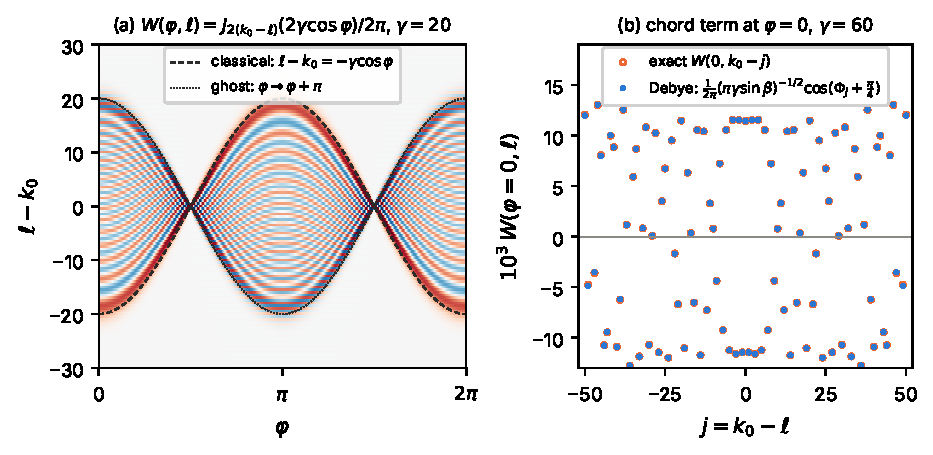
\includegraphics[width=0.95\textwidth]{fig3_wigner.pdf}
\caption{(a) Wigner function of the branch state, Eq.~\eqref{eq:Wbranch}, at $\gamma=20$ (red
positive, blue negative), with the classical curve $\ell-k_{0}=-\gamma\cos\varphi$ and its ghost.
(b) The chord term at $\varphi=0$: exact $W(0,k_{0}-j)=J_{2j}(2\gamma)/2\pi$ (circles) and its
Debye form (dots), oscillating with the fringe phase $\Phi_{j}$.}
\label{fig:wigner}
\end{figure}

\subsection{Smoothing the Wigner function: Husimi distribution}

The smoothing of the previous subsection can be done with coherent states, which turns
$W$ into the Husimi function. On the circle take
\begin{equation}
\ket{\theta,\ell}=\sum_{m\in\mathbb{Z}}\sqrt{g_{\sigma}(m-\ell)}\,e^{-im\theta}\ket m,\qquad
g_{\sigma}(x)=\frac{e^{-x^{2}/2\sigma^{2}}}{\sqrt{2\pi}\sigma},\qquad\ell\in\mathbb{R},
\end{equation}
a packet centred at angle $\theta$ and angular momentum $\ell$, with momentum width
$\sigma$ and angular width $1/2\sigma$. \emph{Resolution of identity:}
$\int_{0}^{2\pi}\frac{\dd\theta}{2\pi}\int\dd\ell\,\ketbra{\theta,\ell}{\theta,\ell}
=\sum_{m}\ketbra mm\int\dd\ell\,g_{\sigma}(m-\ell)=\mathbb{1}$, exactly, with cell $h$.
\emph{Norm:} by Poisson summation,
$\braket{\theta,\ell}{\theta,\ell}=\sum_{m}g_{\sigma}(m-\ell)=1+2\sum_{r\ge1}e^{-2\pi^{2}\sigma^{2}r^{2}}
\cos2\pi r\ell$, within $1.5\%$ of $1$ for $\sigma\ge\frac12$.

For the diagonal $\hat\rho_{1}$ the Husimi function and the Wehrl entropy are
\begin{equation}
Q(\ell)=\bra{\theta,\ell}\hat\rho_{1}\ket{\theta,\ell}=\sum_{m}p_{m}\,g_{\sigma}(\ell-m),\qquad
S_{W}(\sigma)=-\int_{0}^{2\pi}\frac{\dd\theta}{2\pi}\int\dd\ell\,Q\ln Q=-\int\dd\ell\,Q\ln Q,
\end{equation}
i.e.\ the Schmidt weights smoothed by a Gaussian of width $\sigma$. The same smoothing of the
classical density gives $S_{W}[w]\to S_{CE}$ as $\sigma\to0$.

\emph{Bounds.} Let $s(\ell)=\sum_{m}g_{\sigma}(\ell-m)$. Concavity of $\eta(x)=-x\ln x$ (Jensen,
with weights $g_{\sigma}(\ell-m)/s$) gives $\eta(Q)\ge\sum_{m}g_{\sigma}(\ell-m)\eta(p_{m})-Q\ln s$;
integrating over $\ell$, $S_{W}\ge S_{E}-2e^{-2\pi^{2}\sigma^{2}}$ (Wehrl's inequality). Writing
$Q$ as the distribution of $X=M+Z$, with $M\sim p_{m}$ and $Z$ an independent Gaussian,
$h(X)\le H(M)+h(Z)$ gives $S_{W}\le S_{E}+\frac12\ln(2\pi e\sigma^{2})$.

\emph{Deep rotation} (branch quantities; for the parity state every entropy below is
larger by $\ln2$ and the differences are unchanged). Take $p_{j}=J_{j}^{2}=w(1+\cos\Phi_{j})$. Over a stretch of cells where $w$
is constant and $\Phi_{j}\simeq\Phi_{0}+\kappa j$ with $\kappa=-2\beta$, Poisson summation gives
\begin{equation}
\sum_{j}e^{i\kappa j}g_{\sigma}(x-j)=\sum_{r\in\mathbb{Z}}e^{i(\kappa+2\pi r)x}e^{-\sigma^{2}(\kappa+2\pi r)^{2}/2}.
\end{equation}
For $\sigma\gtrsim1$ only the term with the smallest $|\kappa+2\pi r|$ survives, so
\begin{equation}
Q(x)\simeq w\left[1+A\cos\tilde\Phi(x)\right],\qquad A=e^{-\sigma^{2}d^{2}/2},\qquad
d=\min(2\beta,2\pi-2\beta).
\end{equation}
The smoothing lowers the fringe contrast from $1$ to $A$. Averaging over the fast phase
as in Sec.~VI (with $\Delta=h$),
\begin{gather}
S_{W}\simeq S_{CE}^{\rm branch}-\int\dd x\,w\,f(A),\\
f(A)=\big\langle(1+A\cos\Phi)\ln(1+A\cos\Phi)\big\rangle_{\Phi}
=\ln\frac{1+\sqrt{1-A^{2}}}{2}+1-\sqrt{1-A^{2}}
\end{gather}
(Appendix~\ref{app:fA}); $f(1)=1-\ln2$ and $f(0)=0$. With $w\,\dd j=\dd\beta/\pi$ and subtracting
$S_{E}=S_{CE}-(1-\ln2)$,
\begin{equation}
\boxed{\;S_{W}(\sigma)-S_{E}=(1-\ln2)-D(\sigma),\qquad
D(\sigma)=\frac{2}{\pi}\int_{0}^{\pi/2}f\big(e^{-2\sigma^{2}\beta^{2}}\big)\dd\beta\;}
\label{eq:Dsig}
\end{equation}
For $\sigma\gg1$, only $\beta\lesssim1/\sigma$ contributes; expanding $f$ in $A^{2}$ and using
$\int_{0}^{\infty}e^{-4n\sigma^{2}\beta^{2}}\dd\beta=\sqrt\pi/(4\sigma\sqrt n)$,
\begin{equation}
D(\sigma)\simeq\frac{c_{1}}{\sigma},\qquad
c_{1}=\frac{1}{2\sqrt\pi}\sum_{n\ge1}\frac{\binom{2n}{n}}{4^{n}\,2n(2n-1)\sqrt n}=0.080171 .
\end{equation}
Because $A\to1$ near the band edges, where the fringe approximation fails, the
$\gamma^{-1/3}$ correction cancels in $S_{W}-S_{E}$, and Eq.~\eqref{eq:Dsig} holds uniformly in
$\gamma$. Numerically, at $\gamma=10^{4}$: $S_{W}-S_{E}=0.1468,0.2274,0.2675,0.2877$ for
$\sigma=\frac12,1,2,4$, against $(1-\ln2)-D=0.1502,0.2267,0.2668,0.2868$.

\emph{Conclusion.} At fixed $\sigma$, $S_{W}-S_{CE}\to-D(\sigma)\simeq-0.08/\sigma$: the Husimi
entropy lies between $S_{E}$ and $S_{CE}$ and reaches $S_{CE}$ only for $1\ll\sigma\ll\gamma$. The
coherent-state width $\sigma$ is not fixed by the problem; it plays the role of the cell
$\Delta$ in DKS.

%=============================================================================
\section{Summary of results}
%=============================================================================

With $\gamma=\lambda/\hbar|\omega_{1}-\omega_{2}|=\lambda I/\hbar^{2}n=(\lambda/2\hbar)\sqrt{I/\Erel}$:
\begin{itemize}
\item Perturbative reduced density matrix (any $n\neq\pm1,\pm2$):
$\hat\rho_{1}=(1-\epsp-\epsm)\ketbra{m_{1}}{m_{1}}+\epsp\ketbra{m_{1}+1}{m_{1}+1}
+\epsm\ketbra{m_{1}-1}{m_{1}-1}$, $\varepsilon_{\pm}=\lambda^{2}I^{2}/4\hbar^{4}(n\pm1)^{2}$;
$S=\sum_{\pm}\varepsilon_{\pm}\ln(1/\varepsilon_{\pm})+\epsp+\epsm$.
\item Ground state: $S^{0}=-(1-2f)\ln(1-2f)-2f\ln f$, $f=(\lambda I/2\hbar^{2})^{2}$.
\item Classical distribution (exact): $\Wc(\theta_{1},p_{1})=2N/\sqrt{\lambda^{2}-(\Erel-p^{2}/I)^{2}}$;
at weak coupling two arcsine bands of half-width $a=\lambda/|\omega_{1}-\omega_{2}|$,
$N=p_{0}/4\pi^{2}I$.
\item Classical entanglement entropy: $S_{CE}=\ln[2\pi^{2}\lambda/(\Delta|\omega_{1}-\omega_{2}|)]$;
$S_{CE}(\Delta=h)=\ln(\pi\gamma)$.
\item Quantum reduced density matrix (WKB, $\gamma\gg1$, $\Erel\gg\lambda$): eigenvalues
$J_{j}^{2}(\gamma)/2$, each twice; $S_{E}=\ln2-\sum_{j}J_{j}^{2}\ln J_{j}^{2}\to\ln(2\pi\gamma/e)$.
\item Comparison: $S_{CE}-S_{E}=\ln(eh/2\Delta)$; equal for $\Delta=eh/2$; $1-\ln2$ for
$\Delta=h$.
\item Wigner function: integrating over rotor 2 is the partial trace; the reduced Wigner
function is $p_{k}/2\pi$ and its entropy is exactly $S_{E}$. For the WKB branch state
$W_{\rm rel}(\varphi,\ell)=J_{2(k_{0}-\ell)}(2\gamma\cos\varphi)/2\pi$; smoothing it gives the classical
distribution, integrating it keeps the chord term $w\cos\Phi_{j}$, and $1-\ln2$ is the entropy
of the chord terms.
\item Husimi: $S_{W}(\sigma)-S_{E}=(1-\ln2)-D(\sigma)$, $D\simeq0.080/\sigma$; $\sigma$ plays the role of
$\Delta$.
\item Quantum regime of excited states ($\gamma\ll1$):
$S^{n}=-(1-2F)\ln(1-2F)-2F\ln F$, $F=\gamma^{2}/4$; classical regime $S\approx\ln F^{1/2}$.
\end{itemize}

%=============================================================================
\section{Numerical checks}
\label{sec:num}
%=============================================================================

All with $\hbar=I=1$. The classical trajectory uses $\lambda=400$, $\Erel=2500$, $J=0$
($a=4$). Exact eigenstates come from diagonalizing the sector Hamiltonian
$h_{kk'}=k^{2}\delta_{kk'}+\frac{\lambda}{2}(\delta_{k',k+1}+\delta_{k',k-1})$.
\begin{center}
\begin{tabular}{lll}
\hline\hline
quantity & formula & numerics\\
\hline
$\max_{j}|p_{j}-J_{j}^{2}|$, $n=20000$, $\gamma=30$ & 0 & $4.1\times10^{-4}$\\
branch entropy, $n=20000$, $\gamma=30$ & 3.858110 & 3.858114\\
branch entropy, $n=20000$, $\gamma=5$ & 2.271422 & 2.271422\\
$-\sum J_{j}^{2}\ln J_{j}^{2}$ at $\gamma=0.02$ vs Eq.~\eqref{eq:Ssmall} & $2.04205\times10^{-3}$ & $2.04197\times10^{-3}$\\
$-\sum J_{j}^{2}\ln J_{j}^{2}-\ln(\pi\gamma/e)$ at $\gamma=10^{6}$ & $0.965\gamma^{-1/3}=0.00965$ & 0.00966\\
$\ln(\pi\gamma/2)+\sum J_{j}^{2}\ln J_{j}^{2}$ at $\gamma=10^{6}$ vs $1-\ln2$ & 0.306853 & 0.297194\\
classical trajectory: cell weights vs Eq.~\eqref{eq:Wexact} & 0 & $3.7\times10^{-6}$\\
one-band classical entropy ($\Delta=h$): exact vs $\ln(\pi\gamma/2)$ & 1.83788 & 1.84029\\
$p_{0}=1-\epsp-\epsm$, $(m_{1},m_{2})=(4,4)$, $\lambda=0.02$ & 0.99980000 & 0.99980011\\
$S$, $(4,4)$, $\lambda=0.02$, Eq.~\eqref{eq:Sweak} & $2.04207\times10^{-3}$ & $2.04106\times10^{-3}$\\
\quad same without the normalization term & $1.84207\times10^{-3}$ & \\
$S$, $(9,2)$, $\lambda=0.2$, Eq.~\eqref{eq:Sweak} & $4.07805\times10^{-3}$ & $4.07776\times10^{-3}$\\
$\max|W_{\rm rel}-J_{2(k_{0}-\ell)}(2\gamma\cos\varphi)/2\pi|$, $\gamma=6$ & 0 & $2.8\times10^{-16}$\\
$\max_{\ell\in\mathbb{Z}}|\int W\dd\varphi-J_{k_{0}-\ell}^{2}|$ & 0 & $5.6\times10^{-17}$\\
$\max_{\ell\in\mathbb{Z}+\frac12}|\int W\dd\varphi|$ & 0 & $2.1\times10^{-17}$\\
even state: $\max|W-\text{Eq.~\eqref{eq:Weven}}|$ & 0 & $4.2\times10^{-15}$\\
Neumann integral, $n=3$, $\gamma=6$ & 0.0131717822 & 0.0131717822\\
$W(0,k_{0}-j)$, $\gamma=200$, $j=75$: Debye vs exact & $-6.00123\times10^{-3}$ & $-6.00239\times10^{-3}$\\
entropy of reduced Wigner fn.\ vs $S_{E}$ (even, $\gamma=6$) & 3.200465 & 3.200465\\
$S_{W}-S_{E}$, $\gamma=10^{4}$, $\sigma=1$ vs Eq.~\eqref{eq:Dsig} & 0.2267 & 0.2274\\
$\sigma D(\sigma)$ at $\sigma=8$ vs $c_{1}$ & 0.080171 & 0.080171\\
\hline\hline
\end{tabular}
\end{center}

\begin{figure}[h]
\centering
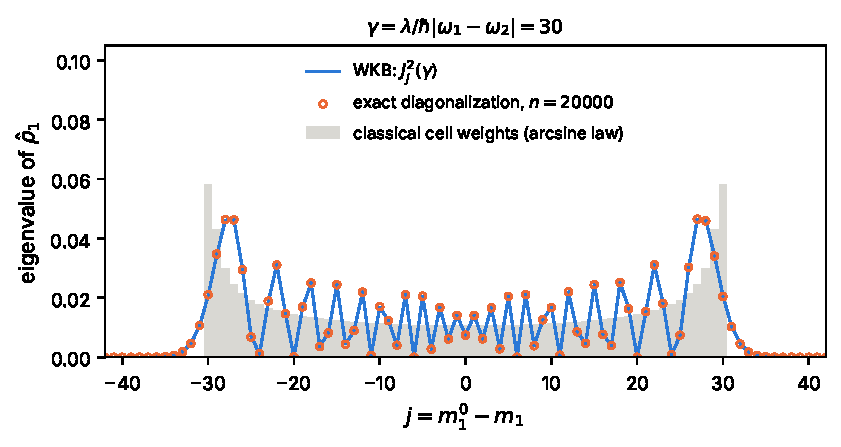
\includegraphics[width=0.75\textwidth]{fig1_weights.pdf}
\caption{Eigenvalues of $\hat\rho_{1}$ for one branch at $\gamma=30$: $J_{j}^{2}(\gamma)$ (line),
exact diagonalization at $n=20000$ (circles), classical cell weights (grey bars).}
\label{fig:weights}
\end{figure}

\begin{figure}[h]
\centering
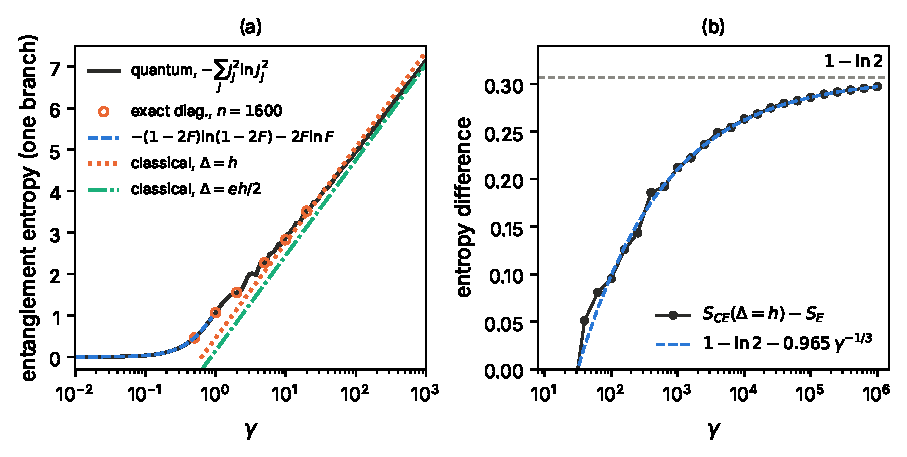
\includegraphics[width=0.95\textwidth]{fig2_entropy.pdf}
\caption{(a) Branch entropy versus $\gamma$: $-\sum J_{j}^{2}\ln J_{j}^{2}$ (solid), exact
diagonalization at $n=1600$ (circles), Eq.~\eqref{eq:Ssmall} (dashed), classical entropy
with $\Delta=h$ (dotted) and $\Delta=eh/2$ (dash-dotted). (b) $S_{CE}(\Delta=h)-S_{E}$
approaching $1-\ln2$ as $\gamma^{-1/3}$.}
\label{fig:entropy}
\end{figure}

\appendix

%=============================================================================
\section{Integrals}
\label{app:int}
%=============================================================================

\emph{1. $\int_{0}^{\pi/2}\ln\cos t\,\dd t=-\frac{\pi}{2}\ln2$.} Let
$I_{c}=\int_{0}^{\pi/2}\ln\cos t\,\dd t=\int_{0}^{\pi/2}\ln\sin t\,\dd t$ (by $t\to\pi/2-t$). Then
\begin{equation}
2I_{c}=\int_{0}^{\pi/2}\ln(\sin t\cos t)\dd t=\int_{0}^{\pi/2}\ln\frac{\sin2t}{2}\dd t
=\frac12\int_{0}^{\pi}\ln\sin v\,\dd v-\frac{\pi}{2}\ln2=I_{c}-\frac{\pi}{2}\ln2,
\end{equation}
using $v=2t$ and $\int_{0}^{\pi}\ln\sin v\,\dd v=2I_{c}$. Hence $I_{c}=-\frac{\pi}{2}\ln2$.
Consequently $\int_{0}^{\pi}\ln\sin\beta\,\dd\beta=-\pi\ln2$ and
$\int_{0}^{\pi}\ln|\cos t|\,\dd t=-\pi\ln2$.

\emph{2. Entropy of the arcsine law.} For $w(j)=1/\pi\sqrt{\gamma^{2}-j^{2}}$ put
$j=\gamma\cos\beta$, so $w\,\dd j=\dd\beta/\pi$ and $\gamma^{2}-j^{2}=\gamma^{2}\sin^{2}\beta$:
\begin{equation}
-\int_{-\gamma}^{\gamma}w\ln w\,\dd j=\frac1\pi\int_{0}^{\pi}\ln(\pi\gamma\sin\beta)\,\dd\beta
=\ln\pi+\ln\gamma-\ln2=\ln\frac{\pi\gamma}{2}.
\end{equation}

\emph{3. Phase average.} Split
$\frac{1}{2\pi}\int_{0}^{2\pi}(1+\cos\Phi)\ln(1+\cos\Phi)\dd\Phi=I_{1}+I_{2}$. With
$1+\cos\Phi=2\cos^{2}(\Phi/2)$ and $t=\Phi/2$,
\begin{equation}
I_{1}=\frac{1}{2\pi}\int_{0}^{2\pi}\ln(1+\cos\Phi)\,\dd\Phi=\ln2+\frac{2}{\pi}\int_{0}^{\pi}\ln|\cos t|\,\dd t
=\ln2-2\ln2=-\ln2 .
\end{equation}
Integrating by parts with $\cos\Phi\,\dd\Phi=\dd(\sin\Phi)$ (the boundary term vanishes),
\begin{equation}
I_{2}=\frac{1}{2\pi}\int_{0}^{2\pi}\cos\Phi\ln(1+\cos\Phi)\dd\Phi
=\frac{1}{2\pi}\int_{0}^{2\pi}\frac{\sin^{2}\Phi}{1+\cos\Phi}\dd\Phi
=\frac{1}{2\pi}\int_{0}^{2\pi}(1-\cos\Phi)\dd\Phi=1 .
\end{equation}
The sum is $1-\ln2$.

\emph{4. The contrast function $f(A)$.}
\label{app:fA}
For $0\le A\le1$ let $s=\sqrt{1-A^{2}}$, $F(A)=\langle\ln(1+A\cos\Phi)\rangle$ and
$G(A)=\langle\cos\Phi\ln(1+A\cos\Phi)\rangle$, averages over $\Phi\in[0,2\pi)$. Then
$f=F+AG$. The standard integral is $F(A)=\ln[(1+s)/2]$, which reduces to item~3 at
$A=1$. Integrating $G$ by parts as in item~3, $G=A\langle\sin^{2}\Phi/(1+A\cos\Phi)\rangle$.
With $u=1+A\cos\Phi$ one has $\sin^{2}\Phi=(A^{2}-1+2u-u^{2})/A^{2}$, and with
$\langle u^{-1}\rangle=1/s$ and $\langle u\rangle=1$,
\begin{equation}
G=\frac{1}{A}\left[\frac{A^{2}-1}{s}+2-1\right]=\frac{1-s}{A},\qquad
f(A)=\ln\frac{1+s}{2}+1-s .
\end{equation}
Expanding instead $(1+y)\ln(1+y)=y+\sum_{k\ge2}(-1)^{k}y^{k}/k(k-1)$ with $y=A\cos\Phi$ and
$\langle\cos^{2n}\Phi\rangle=\binom{2n}{n}4^{-n}$ gives
$f(A)=\sum_{n\ge1}\binom{2n}{n}A^{2n}/[4^{n}2n(2n-1)]=A^{2}/4+A^{4}/32+\dots$, which is used for
$c_{1}$.

%=============================================================================
\section{Bessel functions}
\label{app:bessel}
%=============================================================================

\emph{Jacobi--Anger.} The generating function is
$e^{\frac{z}{2}(t-1/t)}=\sum_{j}J_{j}(z)t^{j}$. With $t=e^{-ix}$,
$\frac12(t-1/t)=\frac12(e^{-ix}-e^{ix})=-i\sin x$, so
$e^{-iz\sin x}=\sum_{j}J_{j}(z)e^{-ijx}$; complex conjugation (real $J_{j}$ for real $z$)
gives $e^{iz\sin x}=\sum_{j}J_{j}(z)e^{ijx}$.

\emph{Neumann identity.} By Parseval,
$\sum_{j}J_{j}^{2}(z)=\frac{1}{2\pi}\int_{0}^{2\pi}|e^{-iz\sin x}|^{2}\dd x=1$.

\emph{Small argument.} $J_{0}(z)=1-z^{2}/4+\dots$, $J_{\pm1}(z)=\pm z/2+\dots$,
$J_{\pm2}(z)=z^{2}/8+\dots$, from the series $J_{j}(z)=\sum_{s}(-1)^{s}(z/2)^{2s+j}/[s!(s+j)!]$
and $J_{-j}=(-1)^{j}J_{j}$.

\emph{Bessel's integral and $\sum_{\nu}J_{\nu}=1$.} Integrating the Jacobi--Anger series
against $e^{i\nu x}$ gives $J_{\nu}(z)=\frac{1}{2\pi}\int_{-\pi}^{\pi}e^{i(\nu x-z\sin x)}\dd x$;
setting $t=1$ in the generating function gives $\sum_{\nu}J_{\nu}(z)=1$. Similarly
$e^{iz\cos x}=\sum_{m}i^{m}J_{m}(z)e^{imx}$.

\emph{Neumann's integral.} $J_{n}^{2}(z)=\frac{1}{\pi}\int_{0}^{\pi}J_{2n}(2z\cos\theta)\,\dd\theta$
(DLMF \S10.9). It is the statement that the momentum marginal of Eq.~\eqref{eq:Wbranch} is
$J_{j}^{2}$.

\emph{Large argument and order (Debye).} For $j=z\cos\beta$, $0<\beta<\pi$, $z\to\infty$:
$J_{j}(z)\simeq\sqrt{2/(\pi z\sin\beta)}\cos(z\sin\beta-j\beta-\pi/4)$; for $|j|>z$, $J_{j}$
decays exponentially (NIST DLMF \S10.19).

\end{document}
